%%%%%%%%%%%%%%%%%%%%%%%%%%%%%%%%%%%%%%%%%
% Journal Article
% LaTeX Template
% Version 1.4 (15/5/16)
%
% This template has been downloaded from:
% http://www.LaTeXTemplates.com
%
% Original author:
% Frits Wenneker (http://www.howtotex.com) with extensive modifications by
% Vel (vel@LaTeXTemplates.com)
%
% License:
% CC BY-NC-SA 3.0 (http://creativecommons.org/licenses/by-nc-sa/3.0/)
%
%%%%%%%%%%%%%%%%%%%%%%%%%%%%%%%%%%%%%%%%%

%%%%%%%%%%%%%%%%%%%%%%%%%%%%%%%%%%%%%%%%%
% WOUT'S STANDARD CODES
%----------------------------------------------------------------------------------------------------------
% INCLUDING A PICTURE
% \begin{figure*}[t]  -> use figure to do a figure in one column, use figure* for two columns. Use [t] for top of page, [b] for bottom, or nothing for in-text
% \includegraphics[width=\textwidth]{setup.png}   -> width can also be put on a number. Using \textwidth maxes it automatically go the entire page.
% \caption{Example of a parametric plot. This caption will be on the bottom.}  -> Caption for the figure
% \end{figure*}
% More info? https://nl.overleaf.com/learn/latex/Inserting_Images
%----------------------------------------------------------------------------------------------------------
% REFERENCING
% In the text:
% \cite{WHO/Europe:2011dg}
% In the reference-list
% \bibitem[WHO/Europe, 2011]{WHO/Europe:2011dg}
% WHO/Europe (2011).
% \newblock Burden of Disease from environmental noise
% \newblock {\em WHO}, ISBN  978 92 890 0229 5.
%----------------------------------------------------------------------------------------------------------
% SECTIONS
% \section{name} for a section
% \subsection{name} for a sub-section
%----------------------------------------------------------------------------------------------------------
% EQUATIONS
% \begin{equation}
% \label{eq:emc}
% e = mc^2
% \end{equation}
%----------------------------------------------------------------------------------------------------------
% FOOTNOTE
% \footnote{Example footnote} -> place this at point where footnote should be in the text
%----------------------------------------------------------------------------------------------------------
% TABLE
% \begin{table}
%\caption{Example table}
% \centering
% \begin{tabular}{llr}
% \toprule
% \multicolumn{2}{c}{Name} \\
% \cmidrule(r){1-2}
% First name & Last Name & Grade \\
% \midrule
% John & Doe & $7.5$ \\
% Richard & Miles & $2$ \\
% \bottomrule
% \end{tabular}
% \end{table}
%%%%%%%%%%%%%%%%%%%%%%%%%%%%%%%%%%%%%%%%%

%----------------------------------------------------------------------------------------
%	PACKAGES AND OTHER DOCUMENT CONFIGURATIONS
%----------------------------------------------------------------------------------------

\documentclass[twoside,twocolumn]{article}

\usepackage{blindtext} % Package to generate dummy text throughout this template 

\usepackage[sc]{mathpazo} % Use the Palatino font
\usepackage[T1]{fontenc} % Use 8-bit encoding that has 256 glyphs
\linespread{1.05} % Line spacing - Palatino needs more space between lines
\usepackage{microtype} % Slightly tweak font spacing for aesthetics

%Extra packages added by A.Gopal
\usepackage{graphicx}
\usepackage[table,xcdraw]{xcolor}
\usepackage{multirow}
\usepackage{makecell}

\usepackage[english]{babel} % Language hyphenation and typographical rules
\usepackage[hyphens]{url}
\usepackage[hmarginratio=1:1,top=32mm,columnsep=20pt]{geometry} % Document margins
\usepackage[hang, small,labelfont=bf,up,textfont=it,up]{caption} % Custom captions under/above floats in tables or figures
\usepackage{booktabs} % Horizontal rules in tables
\usepackage{hyperref}
\usepackage{enumitem} % Customized lists
\setlist[itemize]{noitemsep} % Make itemize lists more compact
\usepackage{float}
\usepackage{abstract} % Allows abstract customization
\renewcommand{\abstractnamefont}{\normalfont\bfseries} % Set the "Abstract" text to bold
\renewcommand{\abstracttextfont}{\normalfont\small\itshape} % Set the abstract itself to small italic text

\usepackage{titlesec} % Allows customization of titles
\renewcommand\thesection{\Roman{section}} % Roman numerals for the sections
\renewcommand\thesubsection{\roman{subsection}} % roman numerals for subsections
\titleformat{\section}[block]{\large\scshape\centering}{\thesection.}{1em}{} % Change the look of the section titles
\titleformat{\subsection}[block]{\large}{\thesubsection.}{1em}{} % Change the look of the section titles

\usepackage{fancyhdr} % Headers and footers
\pagestyle{fancy} % All pages have headers and footers
\fancyhead{} % Blank out the default header
\fancyfoot{} % Blank out the default footer
\fancyhead[R]{Transfer Learning on ACKTR \& PPO  $\bullet$ University of Twente $\bullet$ Jan 2019} % Custom header text
\fancyfoot[RO,LE]{\thepage} % Custom footer text

\usepackage{titling} % Customizing the title section

\usepackage{hyperref} % For hyperlinks in the PDF

%----------------------------------------------------------------------------------------
%	TITLE SECTION
%----------------------------------------------------------------------------------------

\setlength{\droptitle}{-4\baselineskip} % Move the title up

\pretitle{\begin{center}\Huge\bfseries} % Article title formatting
\posttitle{\end{center}} % Article title closing formatting
\title{Performance of ACKTR and PPO with Transfer Learning on Atari-2600 Games} % Article title
\author{%
\textsc{Akarsh Gopal}\\[1ex] % Your name
\normalsize University of Twente \\ % Your institution
\normalsize \href{mailto:a.gopal@student.utwente.nl}{a.gopal@student.utwente.nl} % Your email address
\and % Uncomment if 2 authors are required, duplicate these 4 lines if more
\textsc{Leon van der Neut}\\[1ex] % Second author's name
\normalsize University of Twente \\ % Second author's institution
\normalsize \href{mailto:l.m.b.vanderneut@student.utwente.nl }{l.m.b.vanderneut@student.utwente.nl } % Second author's email address
}
\date{\today} % Leave empty to omit a date
\renewcommand{\maketitlehookd}{%
\begin{abstract}
\noindent In this paper, empirical research is conducted on the effects of Transfer Learning on the performance of two state-of-the-art Reinforcement Learning algorithms in a diverse set of tasks. This is carried out using open-source high-quality implementations of the algorithms presented by OpenAI in Baselines (OpenAIa, 2018). This research intends to develop insights into the effects Transfer Learning bears on the performance of these algorithms and the methodology of research that could be followed to conduct studies which hold significance. The results show positive effects of Transfer Learning on particular source and target task combinations, while also showing negative effects on other combinations. In general, the results show that it is not straightforward to predict when transfer learning will prove beneficial for Reinforcement Learning. 
% Dummy abstract text - replace \blindtext with your abstract text
\end{abstract}
}

%----------------------------------------------------------------------------------------

\begin{document}

% Print the title
\maketitle

%----------------------------------------------------------------------------------------
%	ARTICLE CONTENTS
%----------------------------------------------------------------------------------------
\subsection*{Keywords}
A3C: Asynchronous Advantage Actor-Critic\\
ACKTR: Actor-Critic using Kronecker-Factored Trust Region\\
ALE: Arcade Learning Environment\\
AI: Artificial Intelligence\\
AGI: Artificial General Intelligence\\
CNN: Convolutional Neural Network\\
DL: Deep Learning\\
DNN: Deep Neural Network\\
DRL: Deep Reinforcement Learning\\
DQN: Deep Q Network\\
GPU: Graphics Processing Unit\\
K-FAC: Kronecker-Factored Approximate Curvature\\
MDP: Markov Decision Process\\
PPO(2): Proximal Policy Optimisation\\
RL: Reinforcement Learning\\
TD: Temporal Difference\\
TL: Transfer Learning\\

\section{Introduction}

\textbf{Artificial Intelligence} (AI), a sub-field of Computer Science (Russell \& Norvig, 2003), has been developing rapidly in the last few decades due to the increase in computing power, data collection and breakthroughs made in algorithms since the 1950s (Bostrom, 2014; Kurzweil, 2005). While AI currently casts a spotlight on Deep Learning methods, which are still relatively narrow in their ability to solve problems, the `final` objective is to design an \textbf{Artificial General Intelligence} (AGI) which is defined to be capable of performing intelligently at general tasks much like humans (Baum, 2017; Muehlhauser, 2014). Philosophers and experts in the AI field argue that the advent of AGI would quickly lead to a kind of super-intelligence with an incomprehensible level of intelligence that could lead to either a utopian or dystopian scenario (Bostrom, 2014; Kurzweil, 2005; Muehlhauser and Bostrom, 2014). 

\textbf{Reinforcement Learning} (RL), a sub-field of AI that deals with situations where an `agent` acts in an `environment` , is mainly aimed at creating such an AGI agent that can be implemented across a wide range of activities (Bellemare, Naddaf, Veness \& Bowling, 2013; Sutton \& Barto, 1998). The environment provides feedback to the agent and the agent has a particular goal to achieve within the environment. The objective of RL is to develop methods to allow the agent to learn to achieve the goal while acting within the environment.

RL literature uses a mathematical model of the environment called a \textbf{Markov Decision Process} (MDP) to develop algorithms that learn how to achieve the maximum reward. Using the physical universe as the environment for the RL agent would be computationally intensive, given the complexity of the model required. Doing so would also lead to ethical issues (Bostrom, 2014). Video games follow respective `mechanics` or `physics` that are much simpler than the natural laws that the physical universe seems to follow, as modelled by the scientific field of physics (Einstein, 1916; Hawking \& Stone, 1992; Newton, 1934). Video games also inherently have a main goal to be achieved while playing them. Therefore, learning to play video games can be considered analogous to the learning to achieve a certain goal within the physical universe, motivating RL researchers to use video games as environments for algorithm development (Bellemare et al, 2013). Since the Atari-2600 set of video games presents a diverse and relatively simple set of core tasks, the video games serve well as a platform to research the fundamental characteristics of RL (Mnih, Kavukcuoglu, Silver, Rusu, Veness et al., 2015; Bellemare et al., 2013). 

\textbf{Transfer learning} (TL) is an approach to use `competencies` gained by learning a first, `source` task in improving the learning of a second, `target` task (Weiss, Khoshgoftaar \& Wang, 2016). TL could possibly be used in RL in order to develop and test algorithms that perform well at learning multiple different tasks i.e are generalisable (Laird, Newell, \& Rosenbloom, 1987; Taylor and Stone, 2009), which would be necessary in order to progress towards AGI. This is an active area of research and is the topic of this study. 

The characteristics shown by an algorithm when challenged with TL can be considered `virtual-technological phenomena`. This term is derived from `physical-technological phenomena`, introduced by Boon (2018), which is a term for the objects, properties and processes of an instance, either naturally present or created by mankind. In the virtual realm, which is created by mankind, one can think of this same concept with regard to algorithms.

This study focuses on the virtual-technological phenomena displayed by ACKTR (Wu, Mansimov, Grosse, Liao, \& Ba, 2017) and PPO2 (Schulman, Wolski, Dhariwal, Radford, \& Klimov, 2017) when challenged with TL on specific Atari-2600 games of varying complexity in order to generate insights into the ability of state of the art algorithms to transfer their learning from one task to another. In the process of doing so, the study also intends to possibly develop insights into solutions to improve this generalisability of the algorithms. \textbf{Actor-Critic using Kronecker Factored Trust Region} (ACKTR) and \textbf{Proximal Policy Optimization} (PPO) were chosen for this research since they are considered to be the cutting edge of RL at the moment and implement advanced actor-critic architectures. The specific question addressed by the research is ``What are the effects of Transfer Learning between games on the ability of ACKTR (Wu et al., 2017) and PPO2 (Schulman et al., 2017) to train agents to play Atari 2600 games of varying complexity?''

\textit{The research question is analogous to the situation where a basketball player and a non-athlete are tasked with learning to play football. Intuition would point towards the basketball player being able to pick up the game of football more easily than the non-athlete would.}

%-------------------------------------------------------------------

\section{Theoretical Background}

\subsection*{Reinforcement Learning (RL)}
RL is a sub-field of AI that deals with situations where an `agent` \ acts in an `environment` . The agent has a particular goal to achieve and the environment provides feedback to the agent which can be used to progress towards the agent`s goal. The objective of RL is to develop methods to allow the agent to learn to achieve the goal while acting within the environment. 

The model used for an RL system (Sutton \& Barto, 1998) is as follows: 

An \textbf{agent} interacts with an \textbf{environment} \textit{E} over a number of discrete timesteps. At each time step \textit{t}, the agent receives a \textbf{state} $s_{t}$ and selects an \textbf{action} $a_{t}$ from some\textbf{ set of possible actions} \textit{A} according to its \textbf{policy} $\pi$. Based on the action the agent takes for the particular state, the agent receives the next state $s_{(t+1)}$ and a scalar \textbf{reward} signal $r_{t}$. The process continues until the agent reaches a terminal state after which the process restarts. 

 
\begin{figure}[t]
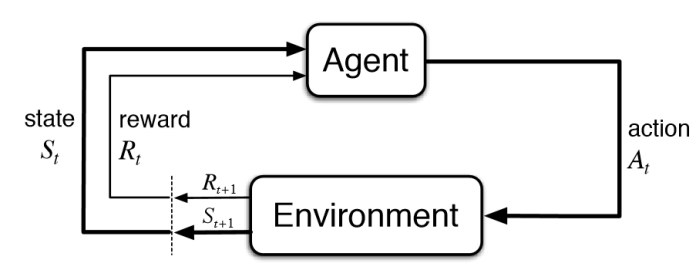
\includegraphics[width=\columnwidth]{fig1.jpg} 
\caption{Diagrammatic Model of Reinforcement Learning (Sutton \& Barto, 1998).}
\end{figure}	

Formally, the RL environment is \textbf{modelled as a Markov Decision Process} (MDP) (Bellman, 1957), which is a 5-tuple:$ <\textit{S},\textit{A},\textit{R},\textit{P},\rho_{0} > $ , where \textit{S} is the set of all valid states, \textit{A} is the set of all valid actions, i.e action space, \textit{R} is the reward function, \textit{P} is the state-transition probability function and $\rho_{0} $ is the distribution of the initial state. The MDP essentially captures all information regarding the environment and the agent in discrete time-steps such that with each step, there is information about the initial state, the current state of the environment, the action taken by the agent at the current state, the reward received by the agent for this action, the probability distribution of the next state based on the current state and the action taken. This means an MDP is a series of blocks of information with each block depending only upon the previous block 

A \textbf{state} \textit{s} is the set of variables which defines the \textbf{environment} at a given time. An \textbf{observation} \textit{o} is a subset or equivalent of the state \textit{s} which is accessible to the agent. Therefore, an observation can also be a partial description of the environment at a given time. When \textit{o} is equivalent to \textit{s}, the environment is said to be fully observable, and when \textit{o} is a subset of \textit{s}, the environment is said to be partially observable. When formally describing algorithms, in RL literature such as Sutton and Barto (1998), state is used instead of observation. Hence, state \textit{s} is used for the rest of the discussion although in practice observation \textit{o} is used. 
\\

N.B. While environments can be deterministic or stochastic, for the sake of simplicity and relevance to the specific environments in this research, we shall focus on stochastic environments only.
\\

An \textbf{Action Space} is the set of all valid actions in a given environment. Action spaces can be discrete, where action spaces are discrete-valued vectors making the number of valid actions finite. Alternatively, they can be continuous which means action space is a real-valued vector. A \textbf{policy} $\pi$ is the rule used by the agent to take an action given an observation, in order to achieve a goal. A stochastic policy maps an action to a state as 
$a_{t} \sim \pi  (*|s_{t})$

A \textbf{trajectory} or an `\textbf{episode}` $\tau$ is a sequence of states and actions in the environment:
$\tau = (s_{0},a_{0},s_{1},a_{1},...) $.
A trajectory is defined by the policy of the algorithm, `choosing` the actions, and the state transition model of the environment, where the state transition model \textit{P} defines the next state given an action-state pair :
$s_{t+1} \sim P(*|s_{t},a_{t})$\\

The \textbf{reward} signal $r_{t} = R(s_{t},a_{t},s_{s+1})$ is a signal produced by the reward function of the environment. This reward signal is provided to the agent, to be used for learning. 

The \textbf{return} is the cumulative reward received by the agent over a \textbf{horizon} (number of timesteps in trajectory) which may be finite or infinite depending on the environment and the trajectory. The goal of RL is to select a policy which \textbf{maximises expected return}. This can be framed as an \textbf{optimisation} problem, wherein a parameterised policy has to be optimised such that the expected return is maximised. Algorithms use approximations of the expected return when optimising their parameters. 

A \textbf{value function} is such an approximation of the expected return of a particular state or state-action pair. Two main value functions (Kimura and Kobayashi, 1998) are: 

\textbf{On-policy value function} approximates the expected return at a state if only a particular policy is followed thereafter: 
\[V^{\pi}(s) = E_{\tau \sim \pi}[R(\tau)|s_{0} = s] \]
\textbf{On-policy action-value function} approximates the expected return at a state if an arbitrary action is taken at a particular state. This is also called the ‘Q’ value ( Watkins \& Dayan, 1992). 
\[ Q^{\pi}(s,a) = E_{\tau \sim \pi}[R(\tau)|s_{0} = s,a_{0}=a] \]
In order to simplify the optimisation problem, each of these value functions can be written as the sum of reward at the current state for the action taken and the value of the rest of the trajectory (Dixit \& Avinash, 1990). This is done using the \textbf{Bellman Equations} (Kirk, 1970). The Bellman equations for each of the two value functions previously mentioned are as follows:
\[ V^{\pi}(s) = E_{a \sim \pi ,\ s^{\prime} \sim P}[r(s,a) + \gamma V^{\pi}(s^{\prime})]\]

\[ Q^{\pi}(s,a) = E_{s^{\prime} \sim P}[r(s,a) + \gamma E_{a\prime \sim \pi}[Q^{\pi}(s^{\prime}, a^{\prime}]] \]

These are used to calculate \textbf{advantage function} $A^{\pi}(s,a)$  is used to mathematically describe how much better a particular action a is for a particular state s, compared to randomly selecting an action according to policy . The advantage function is calculated as:  
\[ A^{\pi}(s,a) = Q^{\pi}(s,a) - V^{\pi}(s) \]
The advantage function is used while optimising the policy in order to decrease variance across updates (Schulman, Levine, Abbeel, Jordan, \& Moritz, 2015).

Most state of the art algorithms since Mnih et al. (2015), including the ones being studied, use \textbf{Deep Reinforcement Learning} (DRL) (Arulkumaran, Deisenroth, Brundage, \& Bharath, 2017). DRL is based on \textbf{Deep Learning} (DL), which is an approach to developing universal approximation functions. It helps develop systems that can produce desired outputs from inputs without having to hand-engineer the transformations in between (Goodfellow et al., 2016; LeCun, Bengio, Hinton, 2015; Schmidhuber, 2015). For a more elaborate explanation of DL, please refer to Appendix A.

The ability of DL to approximate complex functions is useful in the field of RL when the observed state is complex and needs to be mapped to an action output. RL algorithms that use Deep Neural Networks (DNN) are called DRL Algorithms. Recent advances in DL applications motivated the application of DNNs in RL such as in Deep Q Network (DQN) (Mnih et al, 2015). Algorithms such as DQN have raised the standards in test-beds such as the ALE (Bellemare et al., 2013). In DRL algorithms, the policies and/or value estimators are neural networks which are optimised in order to maximise an `objective function`. Specifically, when DRL algorithms obtain images as input, a particular type of DNN called a \textbf{Convolutional Neural Network} (CNN) is used. CNNs use a particular architecture and set of hyperparameters that enable them to excel at image-related tasks. For a more detailed explanation of CNNs, please refer to Appendix A.

\textbf{Hyperparameters} are the parameters that determine the architecture of the network used in the algorithm, like the number of layers of the network, and the specifics of the training process, like proportional step size and learning rate. Proper tuning of these parameters is vital to the performance and stability of the algorithm (Goodfellow, Bengio, Courville, \& Bengio, 2016; Ng, 2017; Sutton \& Barto, 1998).

The algorithms selected for this study perform \textbf{Policy Optimisation}. A parameterised policy $\pi_{\theta}(a|s) $ is to be optimised such that the objective function $J(\pi_{\theta})$ is maximised. This can be done by optimising the parameters via gradient ascent on $J(\pi_{\theta})$. Alternatively, this can be done by maximising local approximations of $J(\pi_{\theta})$. Policy optimisation algorithms also use approximators of value functions and use them in updating the policy (elaboration in Appendix A).

Mathematical Optimisation techniques are used to perform policy optimisation. $J(\pi_{\theta})$ is not necessarily a convex function and therefore can be difficult to optimise with simple gradient ascent, which is a first order optimisation method. In order to ensure global convergence for non-convex problems, \textbf{Trust Region} methods, which are second order optimisation methods, can be used (Yuan, 2015). (elaboration of $1^{st} \ vs \ 2^{nd}$ order optimisation in \hyperref[sec:appx]{Appendix A})
The following algorithms use Trust Region optimisation or a close approximation thereof in order to ensure a `safe` step size and direction.  


\subsubsection*{Actor-Critic Architecture}
In Figure 2 (Patel, 2017) the general setup of the actor-critic model, used in ACKTR and PPO2, is presented. There are two neural networks present, the actor, using a policy-based learning algorithm, and the critic, using a value-based learning algorithm. Both the actor and critic are parameterised according to the CNN architecture proposed by Mnih, Badia, Mirza, Graves, Lillicrap et al. (2016) in OpenAI Baselines (OpenAIa, 2018) implementation of ACKTR as well as in PPO2.

\begin{figure}[t]
	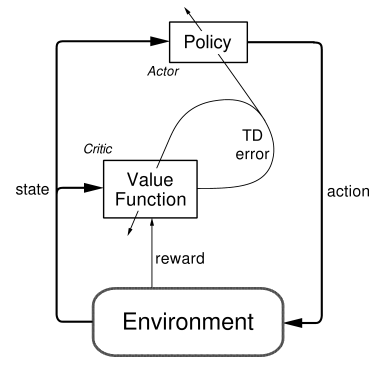
\includegraphics[width=\columnwidth]{fig2.png} 
	\caption{Diagrammatic Model of Actor-Critic Architecture (Patel, 2017).}
\end{figure}

\textit{Actor-critic is analogous to a novice coach and a novice player trying to maximise their combined performance in a particular game. The coach assesses the performance of the player so that the player may improve his skills, while the change in the player`s next performance allows the coach to improve her own assessment of the player. Over time, the coach learns to assess more accurately and the player learns to play better. If the coach is able to assess the player rather well, the player can improve at a faster pace.}

The critic learns to estimate the value of being in a specific state, which is then used to approximate the TD-error and update the value estimation of the critic and the policy of the actor. The Temporal-Difference(TD)-error is the evaluation of the policy of the actor based on the estimation of the reward by the critic and the reward obtained by the policy before the update. TD-error indicates how well the critic can estimate the value of the state based on the actual reward received for the previous action taken by the actor and its estimation of the value of the previous state and its estimation of the value of the previous state. Therefore it is useful in improving both the critic and the actor (Kunz, 2000; Sutton \& Barto, 1998). 

The benefit of using this architecture is that the actor receives feedback from the critic on each action that it takes, whereas the environment only provides feedback on the set of actions performed by the actor during an episode in the form of win or lose, or points gained through the episode depending on the environment the agent operates in. Therefore, the critic creates a more reward-dense environment for the actor, increasing its sample efficiency (in other words, extract a lot of information from relatively little data). In the advantage actor-critic model, the advantage function is used to minimise the variance of both the value estimation performed by the critic and the policy update of the actor, thereby increasing the accuracy of the agent (Mnih et al., 2016).

\subsection*{Algorithms Researched}
\subsubsection*{ACKTR (Wu et al., 2017)}
Actor-Critic using Kronecker-Factored Trust Region (ACKTR, pronounced `actor`) is an algorithm that utilises second-order optimisation to achieve very accurate policy updates and allows the algorithm to achieve a high sample efficiency. ACKTR uses a combination of natural gradient descent (Kakade, 2002), Kronecker-Factored Approximate Curvature (Martens, \& Grosse, 2015) and trust region (Schulman et al., 2015) to update its parameters. 

Natural gradient descent involves computation of the Fisher information matrix. This information matrix represents how probable the estimations produced by the network are using the covariance of the log likelihood of the estimation given the policy: 
\[ F = E_{p(x|\theta)}[\bigtriangledown \log p(x|\theta) \bigtriangledown \log p(x|\theta)^{T}] \]
The inverse of the Fisher matrix, which is required in natural gradient descent, is too heavy to compute because of its sheer size of [$(number \ of \ parameters)^{2}$, $(number \ of \ parameters)^{2}$], considering that the number of parameters in a convolutional neural network often go beyond million (Wu et al., 2017). To work around this, ACKTR uses Kronecker-Factored Approximate Curvature (K-FAC) (Martens, \& Grosse, 2015) in both its actor and critic model, which makes this optimisation computationally feasible. K-FAC uses a number of simplifications to obtain an approximation of the Fisher matrix which works fairly well in practice. The trust region approach of ACKTR ensures that the policy will not adapt too strongly to a single experience by using the approximation of the Fisher matrix to estimate the certainty of the gradient computed to ensure the magnitude of the step-update does not pass the threshold set for uncertainty. ACKTR uses the combination of trust region and K-FAC proposed by Ba, Grosse, \& Martens (2016) and brings this optimization method together with the architecture of \textbf{Asynchronous Advantage Actor Critic} (A3C) (Mnih, et al., 2016). The A3C architecture is a variant of the earlier explained advantage actor-critic model that allows multiple actors to act in an environment simultaneously while updating only one critic model. This is an adaptation that only has an impact on the efficiency of computation and has no implications for the learning of the agent (Mnih et al., 2016). Therefore, this will not be addressed further.

\subsubsection*{PPO (Schulman et al., 2017)}
PPO is a policy optimisation method that empirically performs at least as well as trust region methods but is simpler to implement since it uses a first-order optimisation method. The algorithm effectively uses the same architecture as ACKTR but uses a novel method for policy optimisation: PPO performs stochastic gradient ascent updates on the parameters of the policy in order to maximise a `surrogate` objective function (Achiam, Wu, Morales, Marciniak, Bastovanovicz, Hesse, 2018). The OpenAI Baselines (OpenAIb, 2018) implementation of PPO uses the `clip` \ approach mentioned in Schulman et al. (2017). The surrogate objective function involves a clipping term that helps keep the updated policy parameters close to the previous policy parameters and therefore prevents large step-changes on the policy parameters that may make learning unstable. This allows PPO to make the largest possible update to parameters with the collected data, without compromising learning stability. PPO bypasses the complexity of trust region methods such as ACKTR using this clipping term, without compromising on performance.

In PPO, the advantage is estimated using a value function and a generalised advantage estimation method (Schulman, Moritz, Levine, Jordan, Abbeel, 2015). The algorithm uses a policy network and a value function network to estimate the surrogate objective function. In the case of the Baselines implementation of PPO for Atari games, the policy is a CNN which takes the screen of the game as input and maps this to an action space. 

PPO is an on-policy method that optimises a stochastic policy. At the beginning of the training, the output actions are highly random and this randomness decreases over the training period. This is how the exploration of the state-action-reward space is inherent to the algorithm. However, the policy may get trapped in local optima due to low randomness in action selection in the later stages of training (Achiam et al, 2018).

The Baselines implementation of PPO is called PPO2 because it is a variant that improves performance by using Graphics Processing Units (GPUs) unlike the former, PPO1, which did not do so. PPO will be referred to as PPO2 for the rest of the paper since this is the variant used in the experiments (Achiam et al., 2018).

\subsection*{Environment Used For Study}
The \textbf{Arcade Learning Environment} (ALE) (Bellemare et al., 2013) is an emulator of the Atari-2600 console for video games and is specifically designed to evaluate different algorithms independent of their domain and provides an interface with a large number of Atari-2600 games for testing RL algorithms (Brockman, Cheung, Pettersson, Schneider, Schulman et al., 2016). OpenAI Baselines (OpenAIa, 2018) is a set of high-quality, open-source implementations of the state of the art RL algorithms and supports the ALE as an environment using the OpenAI Gym toolkit (OpenAIb, 2018), which provides an interface between popular RL environments such as the ALE and programming languages such as Python. OpenAI Baselines allows saving of the parameters of the trained model and loading of these weights as initialisation for other runs. It also has a logging feature that stores the total reward per episode of the agent over the 10M timesteps of the run. OpenAI Gym and the ALE can be considered complementary platforms, designed for the objective evaluation and comparison of algorithms and, ALE specifically, for TL as well (Bellemare, et al., 2013; Brockman, et al., 2016). OpenAI Baselines allows state of the art algorithms to be tested on these platforms Therefore OpenAI Baselines and implicitly OpenAI Gym and ALE were used for the study.

The version of ALE used during experimentation has deliberately implemented stochasticity into the Atari-2600 games (Machado, Bellemare, Talvitie, Veness, Hausknecht \& Bowling, 2017) but the Atari-2600 games are deterministic otherwise (Hausknecht \& Stone, 2015). The specific source of stochasticity in the Baselines implementation of (game name)NoFrameskip-v0 is called `sticky actions`, a probability that the action of the previous frame is repeated in the current frame instead of the inputted action. In this case, the probability that an action would be `sticky` was set 0.25 (OpenAIa, 2018), in accordance with the suggestion from Machado et al. (2017).

\subsection*{Transfer Learning (TL)}
Transfer Learning is the process of improving learning performance in a particular`target` task having already learned to perform a related, but different, `source` task (Taylor \& Stone, 2009). Psychological literature studies TL in humans and develops ideas analogous to TL in Machine Learning research (Thorndike \& Woodworth, 1901; Skinner, 1953).

Collection of training data for physical-world applications can be prohibitively expensive or practically impossible in many cases. TL can help reduce the need and effort to collect this training data in such cases (Pan \& Yang, 2010). This has been shown to work well in DL applications such as computer vision and speech recognition (Hoo-Chang, Roth, Gao, Lu, Xu et al., 2016; Weiss et al., 2016). The insight behind TL is that generalisation may occur not only within tasks but also across tasks (Taylor \& Stone, 2009). TL research could also become relevant in transferring learning from virtual simulation (source task) to the physical world (target task) applications like robotics, as demonstrated by (Andrychowicz, Baker, Chociej, Jozefowicz, McGrew et al., 2018). 

It is also important to note that TL can have a detrimental effect on the performance of the learner and this phenomenon is called negative transfer (Weiss et al., 2016). This can occur in cases where the source task and target task differ significantly. Negative transfer in the context of RL has been recorded by Glatt, Silva \& Costa (2016) where the source task and target task were video games with different mechanics. In order to effectively apply TL, the source and target task selection must, therefore, be compatible, i.e there should be at least a non-negative effect of TL. 

Challenges in TL that require further research include the handling of negative transfer and the determination of suitability of a source and target task pair for transfer (Glatt et al., 2016). Glatt et al. (2016) defined the similarity of the learned tasks subjectively and stated that this procedure was not appropriate for a general case since a complete understanding of how neural networks generalise tasks is lacking, and human intuition can go wrong in such situations. Therefore, developing a framework for defining the similarity of the tasks is another challenge in TL.

\begin{figure*}[]
	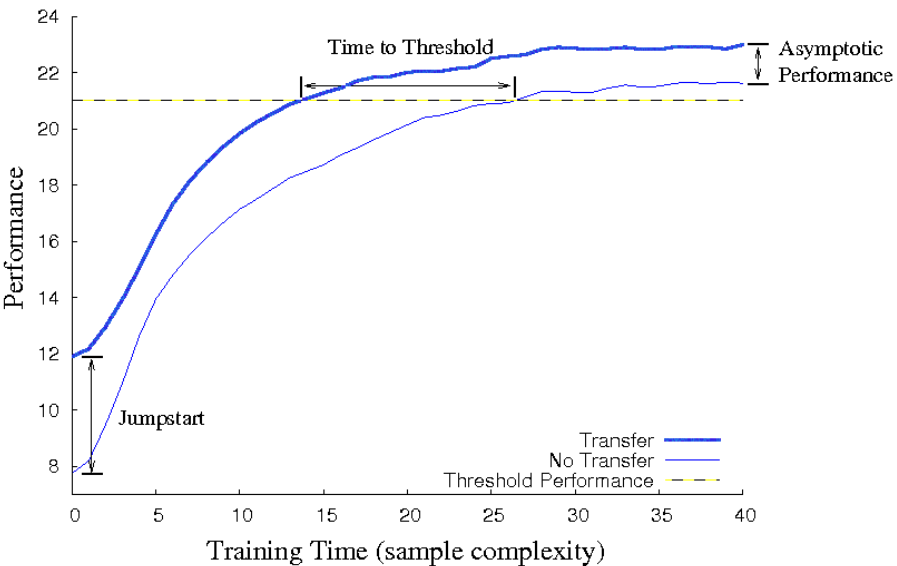
\includegraphics[width=\textwidth]{fig3.png} 
	\caption{Possible Metrics of TL in RL (Taylor \& Stone, 2009).}
\end{figure*}

The definition of evaluation metrics for TL is also a challenge because there are several possible metrics (Taylor \& Stone, 2009).
Taylor and Stone (2007) defined and used the following metrics (represented visually in Figure 3) in a cross-domain TL study:
 \begin{enumerate}
	\item \textbf{Jumpstart}: The difference in the initial performance of the agent in the target task with respect to that in the source task could indicate whether the agent has acquired useful priors.
	\item \textbf{Asymptotic Performance}: The difference between the asymptotic performances of the agent in the two (target and source) tasks could indicate whether the agent reaches a higher final score.
	\item \textbf{Total Reward}: The difference in the total returns gained by an agent over each of the two tasks could indicate the effect of transfer over the span of the task(s).
	\item \textbf{Transfer Ratio}: The ratio of the total returns gained by the agent in the two tasks could also indicate the overall effect of TL for the source and target task pair.
	\item \textbf{Time-to-Threshold}: The difference in the time needed by the agent to achieve a specified performance threshold in the two tasks could indicate whether the speed of learning has changed due to transfer.
\end{enumerate}

\subsection*{Hypothesis}
Combining the discussed theory of RL, TL, and the intuition that similar tasks would have similar underlying `mechanics` such that the algorithms can transfer competencies learned from one task to the other beneficially, we develop our hypothesis:

\textit{TL decreases training time (number of time-steps taken for the agent to achieve a threshold of return) for games that are similar when compared to directly training on the target task. Also, we hypothesize that training time for similar games is lesser than training times for dissimilar games.}

The results of testing this hypothesis can be compared with the prediction made in the hypothesis to verify or disprove the hypothesis. Since the phenomenon being considered for the study is a virtual-technological phenomenon and is essentially a simulation in and of itself, our hypothesis makes a claim regarding the performance of the model (agent) in the larger system (environment(s)). 

\section{Methodology}
The method we developed to test the effects of TL on the performance of algorithms for combinations of games is as follows:
\subsection*{Setup}
A set of 4 games were selected, the paired combinations of which were used as source tasks and target tasks. The selection of games was restricted to games with the same action space since a different action space would require to adapt the network architecture in the process of transfer and this would complicate the process. From these games, the Atari-2600 games Q*Bert, Pong, Demon Attack, and Space Invaders were chosen. Atari-2600 games were specifically chosen since they are widely used in the field of RL to compare different algorithms (Mnih et al., 2016; Mnih, Kavukcuoglu, Silver, Graves, Antonoglou et al., 2013; Wu et al., 2017; Schulman et al., 2017; Van Hasselt, Guez, \& Silver, 2016) and since the selection of games researched has to allow testing of the hypothesis. This was chosen on the basis of conceptual similarity of two similar games, Space Invaders, Demon Attack, one simple game with one big contrast (not avoid the object coming at the moveable instance but bounce it instead) Pong, and one vastly different game, Q*Bert. 
\begin{figure}[t]
	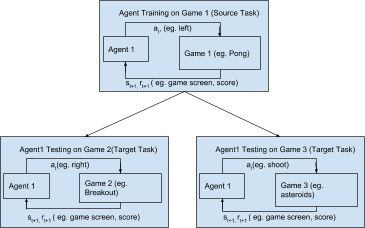
\includegraphics[width=\columnwidth]{fig4.png} 
	\caption{Diagrammatic representation of experiment.}
\end{figure}
The literature for video-game complexity analysis was deemed to be scarce and under-developed, after performing an extensive search and consulting Bellemare, Veness, \& Bowling (2012); Brockman, et al. (2016); Guo, Singh, Lee, Lewis, \& Wang (2014); Levine, Bates Congdon, Ebner, Kendall, Lucas, Miikkulainen, ... \& Thompson (2013); Mnih, Kavukcuoglu, Silver, Rusu, Veness, ... \& Petersen (2015), and Wolf (2013). 

The complexities of these video games were therefore assessed using criteria selected mainly based on the intuition, in order to qualitatively define the conceptual complexities of the video games. The conceptual similarity between any two of the selected games was assessed using their respective conceptual complexities. Criteria include \textbf{Color Scheme, Background Color, Degrees of Freedom, Score Scale, Action space, Movement Orientation, Opponents, Behavior of opponent, Objective of player, Human-Level performance in the game (threshold)} 

\subsection*{Experiments}
First, one algorithm was trained on all four games with randomly initialised models, thus acquiring `base` models for each game for that algorithm. This resulted in 4 trained models and logs. These training runs will be referred to as baseline runs for simplicity. Next, Table 1 (Columns 2-5) was followed for both algorithms, generating 12 transfer models and logs. These runs will be referred to as transfer runs for simplicity. Therefore 16 logs were collected for one algorithm. The same runs were executed twice to inspect the stochasticity present in the system. All runs of the second round of TL used the same base model as the first round, in order to test the stochasticity of the results of the transfer runs. To check whether the procedure executed to transfer the model from one run to the other, `self-transfer` runs were conducted such that the source task and target task were the same. The self-transfer runs were run only once for each game since it is assumed that there is no stochasticity present in the procedure executed. This process was repeated for the other algorithm (See Appendix B). 

To create a good overview of how ACKTR and PPO2 behave in TL all possible combinations of base model and the game played were considered for both algorithms. A matrix of the combination of source task and target task was developed, which is the same for both algorithms (Table 1). Each run consists of a variable number of game episodes from which the algorithm learns, since the episode can last from 0 timesteps to tmax (10 Million timesteps), depending on how well the algorithm performs. To avoid varying amounts of training data, the number of timesteps (the decisions taken by the algorithm) of training was set at 10M timesteps. This number of timesteps is commonly used to measure the performance of reinforcement learning algorithms (Mnih et al. 2015; Schulman et al., 2017; Wu, 2017) 
\begin{table*}[]
	\begin{tabular}{l|p{2.2cm}p{2cm}p{2cm}p{2cm}p{1.2cm}}
		\hline
		\multicolumn{6}{c}{Runs Executed}                                                                   \\ \hline
		Base model (Source Task) & Base model (Source Task) & Q*Bert & Pong & \makecell{\\Space \\ Invaders} & Demon Attack \\
		\hline
		Game played(Target task) &                          &        &      &                &              \\
		\rowcolor[HTML]{EFEFEF} Q*Bert (QB)              & x2                       & x1     & x2   & x2             & x2           \\
		Pong (PO)                & x2                       & x2     & x1   & x2             & x2           \\
		\rowcolor[HTML]{EFEFEF} Space Invaders (SI)      & x2                       & x2     & x2   & x1             & x2           \\
		Demon Attack (DA)        & x2                       & x2     & x2   & x2             & x1           \\ \hline
	\end{tabular}
	\caption{Distribution of Initializations of each Game and the Game that it was Subsequently Transferred to Completed for both ACKTR and PPO2. The `x2` within the cells says that each of the training runs was run twice. Cells with `x1` refer to the self-transfer runs.}
\end{table*}

The Baselines implementation of PPO2 and ACKTR from OpenAI (OpenAIa, 2018) were used in this experiment to ensure a stable and thoroughly tested implementation of the algorithms. 
The same software-environment was used for all the runs to avoid any unnecessary variables that could influence the experiment.
Hyperparameters of the algorithms were not changed from the default Baselines implementation (OpenAI, 2018) and can be found in Appendix B. The computer hardware specifications such as processor clock speed, computer memory, and GPU memory affect the speed of training. The higher the specifications of this hardware, the faster is the training. Due to limitations in available equipment and time, two devices had to be used to carry out all training runs. As seen in Figure 5, the virtual technological phenomena being studied relies on a hierarchy of software and hardware. 

\begin{figure}
	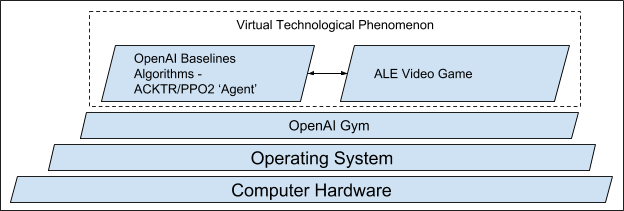
\includegraphics[width=\columnwidth]{fig5.png} 
	\caption{Dependency hierarchy of the studied phenomena. The underlying layers had to be kept constant in order to ensure reproducibility of the phenomena}
\end{figure}

In order to ensure reproducibility and maintain uniformity in the context of phenomena (Figure 5) between the two devices used, it was ensured that the hardware specifications were similar. The relevant software specifications of the two devices such as Operating System and the particular versions of OpenAI Gym, Baselines were also the same. For the specifics on the hardware and software setup, see Appendix B.

\subsection*{Analysis}
The following metrics were chosen based on suggestions by Taylor and Stone (2009) and measured for each run: 
\begin{enumerate}
	\item \textbf{Time-to-Threshold}. Human-level performance listed for games in the DQN paper (Mnih et al. 2015) taken as the threshold. This is calculated by finding the average of the time at which the two runs reach the threshold. In cases where both runs have not reached the threshold, this data is left black. However, in cases where just one run reaches the threshold, the time is approximated by finding the time at which the average score of the two runs reaches the threshold(if it does). This had to be done manually and is prone to error in the order of $10^{5}$ timesteps.
	\item \textbf{Score at time-to-threshold for the base model}. The score achieved by transfer runs at the time at which the baseline run achieves the threshold. This metric is used to check whether the transfer runs are lagging or leading with respect to the baseline run.
	\item \textbf{Mean reward}. This is effectively the mean reward accumulated by the algorithm throughout the run, providing insight into the overall learning.
	\item \textbf{Standard Deviation}. This is measured as the mean of the 500-point rolling standard deviations of the algorithm throughout the training run. This provides insight into how much the scores vary over the training.
	\item \textbf{Scores at 0M, 2.5M, 5M, 7.5M and 9.9M timesteps}. M stands for Million.
	\begin{itemize}
		\item 0M. This is measured by finding the 500-point rolling average of the first 500 episodes and helps in measuring the jumpstart (Taylor \& Stone, 2009)
		\item 2.5M, 5M, and 7.5M These are the 500-point rolling averages of scores at each of these times respectively, providing insight into the algorithms`s training.
		\item 9.9M. This is measured by finding the 500-point rolling average of the score at 9.9M timesteps. This indicates asymptotic performance (Taylor \& Stone, 2009)
	\end{itemize}
\end{enumerate}

\begin{figure*}[h]
	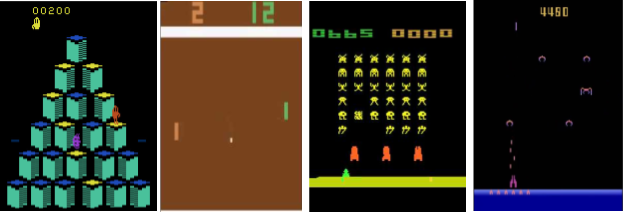
\includegraphics[width=\textwidth]{fig6.png} 
	\caption{Screenshots of the four selected games. From left to right: Q*Bert, Pong, Space Invaders and Demon Attack.}
\end{figure*}

The 500-point rolling average is the average of the current and previous 499 episode scores achieved by the algorithm. The 500-point rolling standard deviation is the standard deviation of the current and the previous 499 episode scores achieved by the algorithm

The average of each of these metrics for the twin runs was used as an estimate of the mean. However, it is important to note that the mean 500-point rolling standard deviation is large and the sample size n, is just 2, therefore results are not statistically significant. 

Metrics (5) were then normalised with the range (threshold, min game score) in order to be able to compare effectively, as suggested by Bellmaire et al (2013). This was done as follows: norm(metric) = (metric - min score)/(threshold - min score) 
This enabled comparison of the effects of transfer learning across algorithms and games.

The effects of TL were then assessed as positive if a majority of the above metrics were better than the baseline metrics for a particular target task. Effects were considered negative if a majority of the above metrics were worse than the baseline metrics for that target task. The mean reward was used as a tiebreaker.


%------------------------------------------------

\section{Results}

\subsection*{Game Complexity}

\begin{table*}[]
	\begin{tabular}{p{2cm} p{3cm}p{3cm}p{3cm}p{3cm}}
	\hline
	\multicolumn{5}{c}{\textbf{Game Complexity}} \\
	\hline
	& \multicolumn{1}{c}{\textbf{Q*Bert}} & \multicolumn{1}{c}{\textbf{Pong}} & \multicolumn{1}{c}{\textbf{Space Invaders}} & \multicolumn{1}{c}{\textbf{Demon Attack}} \\
	\rowcolor[HTML]{EFEFEF} 
	\textbf{Color Scheme} & Black, Yellow, Navy Blue, Sky Blue, Red, & Brown, Red, Green, White & Black, Yellow, Green, Orange & Black, Yellow, Purple, Navy Blue \\
	\textbf{Background Color} & Black & Brown & Black & Black \\
	\rowcolor[HTML]{EFEFEF} 
	\textbf{Degrees of Freedom} & 3 & 1 & 2 & 2 \\
	\textbf{Score Scale} & {[}0,Inf) & {[}-21,21{]} & {[}0,Inf) & {[}0,Inf) \\
	\rowcolor[HTML]{EFEFEF} 
	\textbf{Action space} & Discrete(6) & Discrete(6) & Discrete(6) & Discrete(6) \\
	\textbf{Movement Orientation} & Vertical and Horizontal /Diagonal movement & Vertical movement only & Horizontal movement only & Horizontal Movement only \\
	\rowcolor[HTML]{EFEFEF} 
	\textbf{Opponents} & Present & Present & Present & Present \\
	\textbf{Behavior of opponent} & Opponent attempts to block the player in various ways & Attempt to return to ball & Move from left to right while shooting at the player. Move one down when reaching the edge. & Move left, right, up and down in an irregular pattern while shooting at the player \\
	\rowcolor[HTML]{EFEFEF} 
	\textbf{Objective of player} & Avoid opponent, while activating all tiles & Bounce ball past opponent & Shoot all opponents before the opponents reach the ground while avoiding fire & Shoot all opponents before opponents reach the ground while avoiding fire \\
	\textbf{Human Level performance (threshold score)} & 13455 & 9.3 & 1652 & 3401 \\
	\hline
\end{tabular}
\caption{Conceptual complexity of the games are described using the above features as visible on the game screens.}
\end{table*}


As seen in Figure 6 and defined in Table 2, the games differ in colour schemes and game mechanics. However they share the same (discrete) action space of dimension 6: [ 0: ``NOOP'', 1: ``FIRE'', 2: ``UP'', 3: ``RIGHT'', 4: ``LEFT'', 5: ``DOWN'']. 

Demon Attack and Space Invaders are conceptually very similar, they have the same objectives, same degree of freedom, and similar objectives. 
Q*Bert is conceptually different from all other games and is conceptually more complex since it has a higher degree of freedom, a larger set of colours and an opponent with behavior adapted to the player. Pong is less complex than the other games, it has the least degrees of freedom, a simple objective, and predictable behavior of the opponent. 
Demon Attack seems to be the most complex game visually, considering it includes some simple animation and irregular patterns of opponents.

\subsection*{Experiments}
From the experiments, the reward achieved by the agent at the end of each episode and the timesteps elapsed in each episode were logged for each run of 10M timesteps. The following plots visualise the reward per episode for all runs of a [game, algorithm] pair over the 10M timesteps. The various curves within the plots represent the different initialisations of the models, allowing us to visually inspect the effects of TL. The raw data is prone to noise and is unintelligible (Presented in Appendix B). In order to solve this, the 500-point rolling average of each trial is presented in Figure 7.

\begin{figure*}
	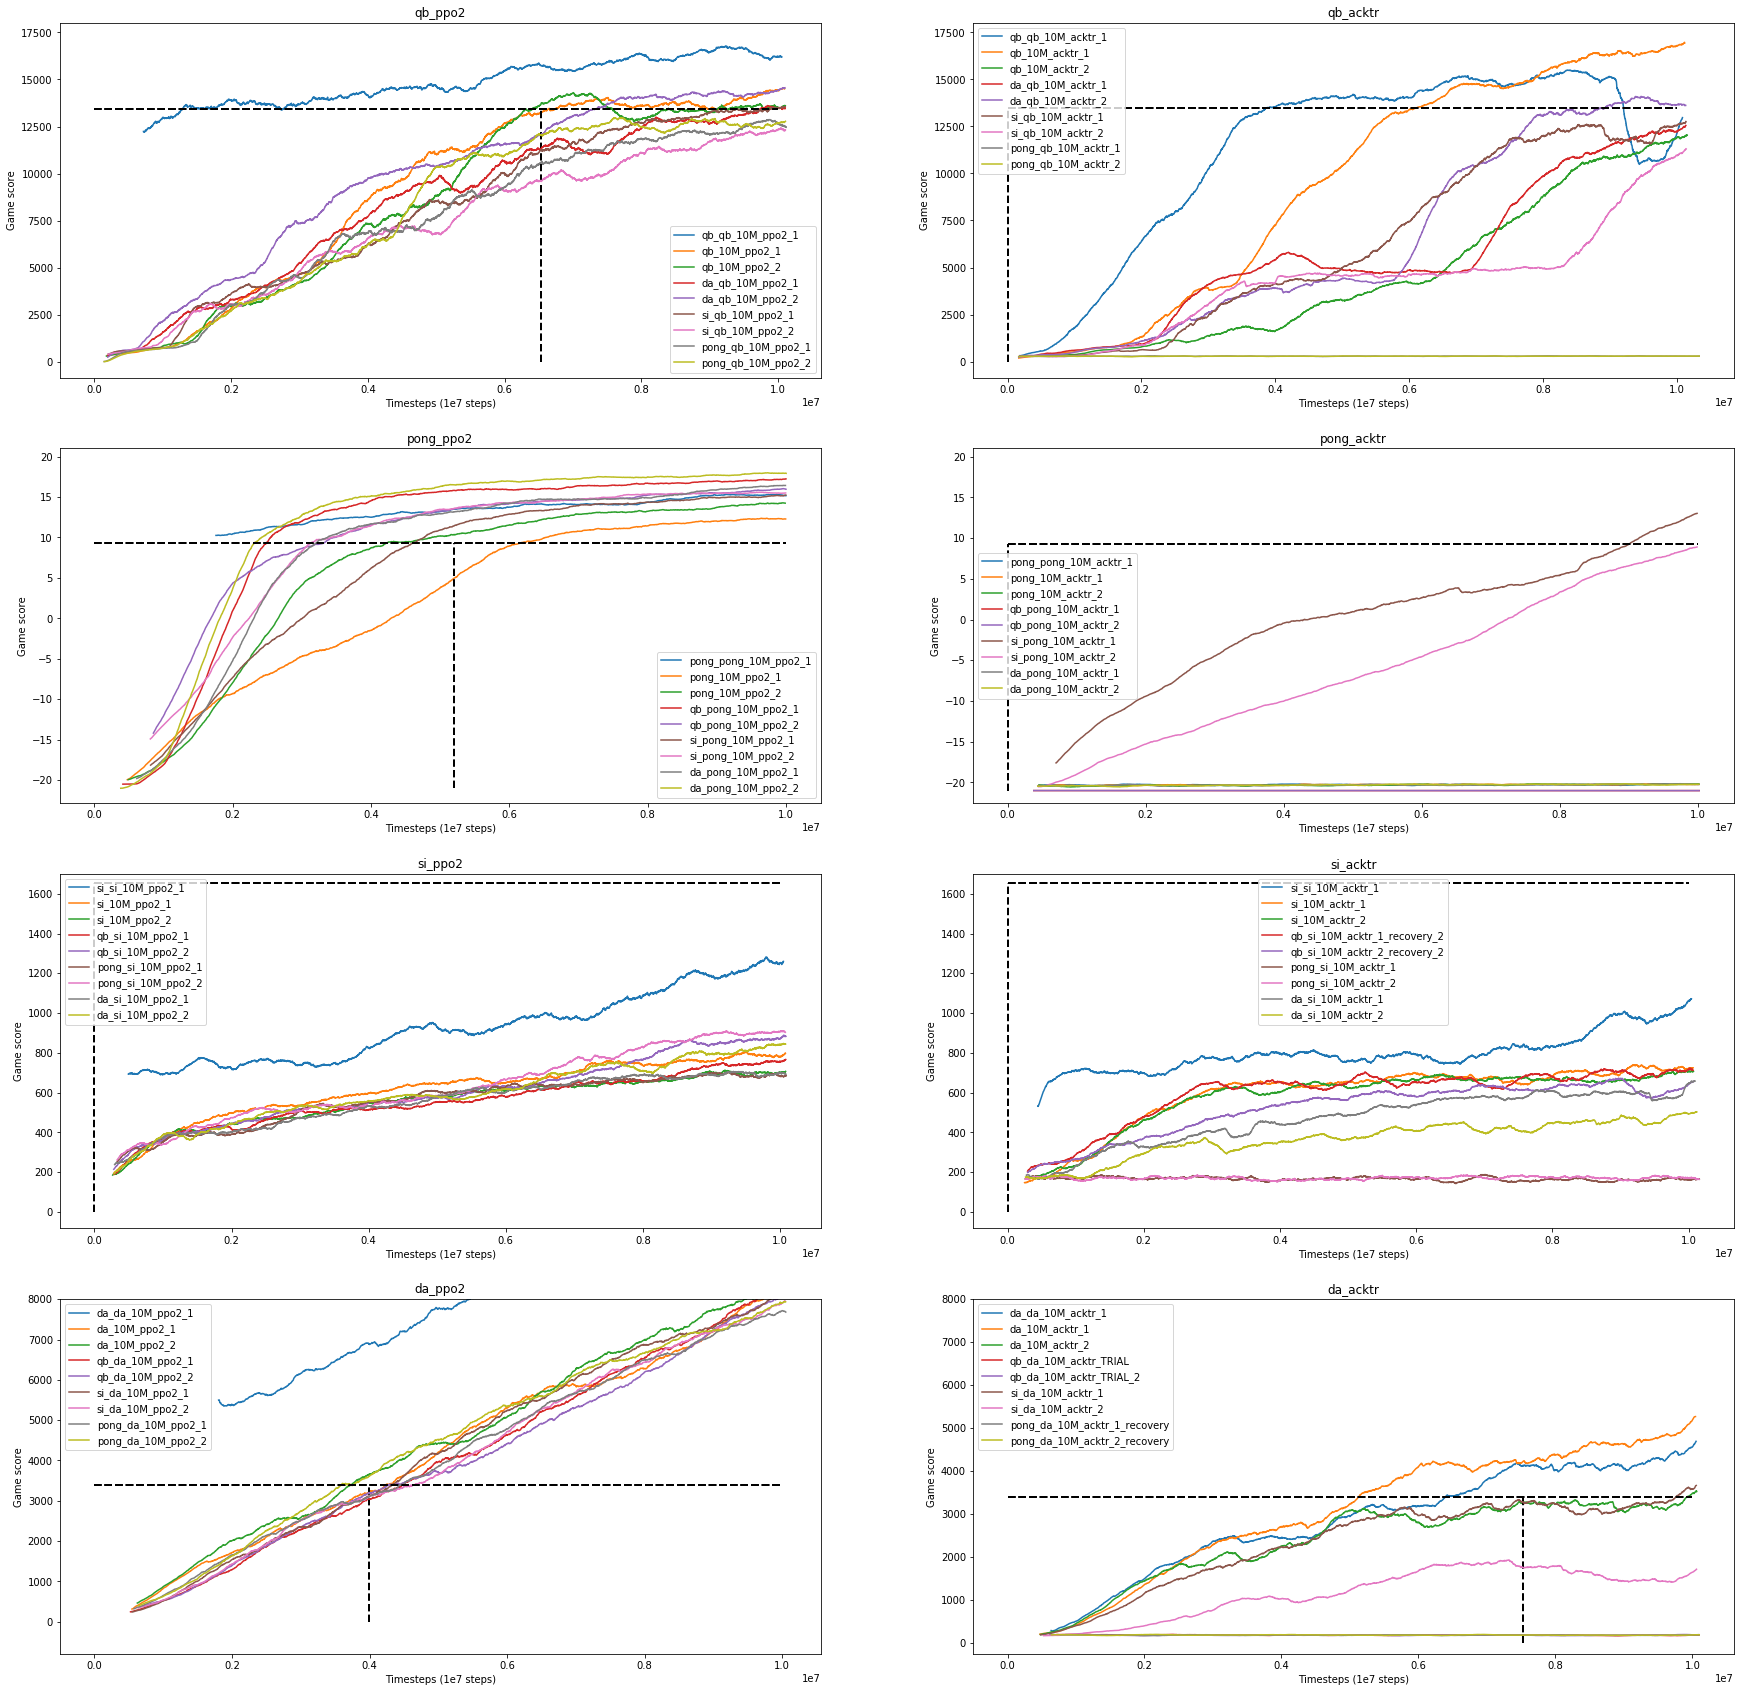
\includegraphics[width=\textwidth]{fig7.png} 
	\caption{500-Point rolling average of the game score plotted against the 10M timesteps. The hyphenated lines superimposed onto these graphs represents the thresholds (human level performance). Each column of graphs represents an algorithm, as PPO2 and ACKTR runs from left to right respectively. Each row of graphs represents a game as Q*Bert, Pong, Space Invaders and Demon Attack from top to bottom respectively. The titles of the graphs follow the naming convention: game\_algorithm. The legend follows the naming convention: source-game\_target-game\_number-of-timesteps\_algorithm\_run-number}
\end{figure*}

\begin{table*}[]
	\begingroup
	\renewcommand{\arraystretch}{1.2}
	\begin{tabular}{p{1.3cm}p{1cm}p{0.9cm}p{1cm}p{1.3cm}p{1.2cm}p{1.2cm}p{0.7cm}p{0.7cm}p{0.7cm}p{0.7cm}p{0.7cm}}
		\hline
		\multicolumn{12}{c}{Results of Experiments} \\
		\hline
		&  &  &  &  &  &  & \multicolumn{5}{c}{\thead{Normalised Score}} \\
		\multirow{-2}{*}{\thead{Target task}} & \multirow{-2}{*}{\thead{Source\\ task}} & \multirow{-2}{*}{\thead{Algorithm}} & \multirow{-2}{*}{\thead{Time-to\\-threshold\\(timesteps)}} & \multirow{-2}{*}{\thead{Reward at \\time-to\\-threshold\\ of baseline run}} & \multirow{-2}{*}{\thead{Mean\\ Reward}} & \multirow{-2}{*}{\thead{Standard\\ deviation}} & \textbf{0M} & \textbf{2.5M} & \textbf{5M} & \textbf{7.5M} & \textbf{9.9M} \\
		\hline
		\rowcolor[HTML]{EFEFEF} 
		\cellcolor[HTML]{EFEFEF} & - & \cellcolor[HTML]{EFEFEF} & \textbf{6532761} & \textbf{13471.05} & 6836.744 & 2639.221 & 0.024 & 0.273 & 0.737 & \textbf{1.023} & \textbf{1.039} \\
		\rowcolor[HTML]{EFEFEF} 
		\cellcolor[HTML]{EFEFEF} & DA & \cellcolor[HTML]{EFEFEF} & 8549481 & 13462.625 & \textbf{7493.368} & 2583.759 & 0.021 & \textbf{0.348} & \textbf{0.746} & 0.92 & 1.037 \\
		\rowcolor[HTML]{EFEFEF} 
		\cellcolor[HTML]{EFEFEF} & SI & \cellcolor[HTML]{EFEFEF} & - & - & 6321.353 & 2714.467 & \textbf{0.03} & 0.28 & 0.57 & 0.828 & 0.955 \\
		\rowcolor[HTML]{EFEFEF} 
		\cellcolor[HTML]{EFEFEF} & Pong & \multirow{-4}{*}{\cellcolor[HTML]{EFEFEF}PPO2} & - & - & 6124.969 & 2486.774 & 0.001 & 0.265 & 0.669 & 0.899 & 0.942 \\
		\rowcolor[HTML]{C0C0C0} 
		\cellcolor[HTML]{EFEFEF} & - & \cellcolor[HTML]{C0C0C0} & \textbf{9000000*} & \textbf{13460*} & \textbf{4805.455} & 1598.237 & 0.017 & 0.147 & \textbf{0.508} & \textbf{0.818} & \textbf{1.059} \\
		\rowcolor[HTML]{C0C0C0} 
		\cellcolor[HTML]{EFEFEF} & DA & \cellcolor[HTML]{C0C0C0} & - & - & 4317.195 & 1418.888 & \textbf{0.02} & \textbf{0.158} & 0.346 & 0.735 & 0.965 \\
		\rowcolor[HTML]{C0C0C0} 
		\cellcolor[HTML]{EFEFEF} & SI & \cellcolor[HTML]{C0C0C0} & - & - & 3754.789 & 1491.958 & 0.018 & 0.118 & 0.355 & 0.62 & 0.864 \\
		\rowcolor[HTML]{C0C0C0} 
		\multirow{-8}{*}{\cellcolor[HTML]{EFEFEF}Q*Bert} & Pong & \multirow{-4}{*}{\cellcolor[HTML]{C0C0C0}ACKTR} & - & - & 285.993 & 111.914 & 0.019 & 0.021 & 0.022 & 0.021 & 0.021 \\
		\rowcolor[HTML]{EFEFEF} 
		\cellcolor[HTML]{C0C0C0} & - & \cellcolor[HTML]{EFEFEF} & 5192064 & 7.614 & 1.73 & 5.202 & 0.035 & 0.546 & 0.924 & 1.092 & 1.131 \\
		\rowcolor[HTML]{EFEFEF} 
		\cellcolor[HTML]{C0C0C0} & QB & \cellcolor[HTML]{EFEFEF} & 2900590 & \textbf{10.059} & \textbf{8.993} & 3.865 & 0.122 & \textbf{0.967} & 1.171 & 1.21 & \textbf{1.239} \\
		\rowcolor[HTML]{EFEFEF} 
		\cellcolor[HTML]{C0C0C0} & SI & \cellcolor[HTML]{EFEFEF} & 3868794 & 8.221 & 7.528 & 4.289 & \textbf{0.148} & 0.693 & 1.096 & 1.173 & 1.199 \\
		\rowcolor[HTML]{EFEFEF} 
		\cellcolor[HTML]{C0C0C0} & DA & \multirow{-4}{*}{\cellcolor[HTML]{EFEFEF}PPO2} & \textbf{2760533} & 8.884 & 8.698 & 4.405 & 0.02 & 0.917 & \textbf{1.175} & \textbf{1.224} & 1.26 \\
		\rowcolor[HTML]{C0C0C0} 
		\cellcolor[HTML]{C0C0C0} & - & \cellcolor[HTML]{C0C0C0} & - & - & -20.303 & 0.837 & 0.022 & 0.021 & 0.023 & 0.025 & 0.025 \\
		\rowcolor[HTML]{C0C0C0} 
		\cellcolor[HTML]{C0C0C0} & QB & \cellcolor[HTML]{C0C0C0} & - & - & -21 & 0 & 0 & 0 & 0 & 0 & 0 \\
		\rowcolor[HTML]{C0C0C0} 
		\cellcolor[HTML]{C0C0C0} & SI & \cellcolor[HTML]{C0C0C0} & 9650000* & - & \textbf{-4.271} & 4.435 & \textbf{0.064} & \textbf{0.343} & \textbf{0.587} & \textbf{0.786} & \textbf{1.047} \\
		\rowcolor[HTML]{C0C0C0} 
		\multirow{-8}{*}{\cellcolor[HTML]{C0C0C0}Pong} & DA & \multirow{-4}{*}{\cellcolor[HTML]{C0C0C0}ACKTR} & - & - & -20.312 & 0.834 & 0.019 & 0.021 & 0.023 & 0.024 & 0.025 \\
		\rowcolor[HTML]{EFEFEF} 
		& - & \cellcolor[HTML]{EFEFEF} & - & - & 560.944 & 184.444 & 0.115 & \textbf{0.301} & \textbf{0.369} & 0.426 & 0.446 \\
		\rowcolor[HTML]{EFEFEF} 
		& QB & \cellcolor[HTML]{EFEFEF} & - & - & 556.744 & 176.388 & 0.122 & 0.285 & 0.341 & 0.414 & \textbf{0.491} \\
		\rowcolor[HTML]{EFEFEF} 
		& Pong & \cellcolor[HTML]{EFEFEF} & - & - & \textbf{570.029} & 186.469 & \textbf{0.155} & 0.288 & 0.361 & \textbf{0.434} & 0.484 \\
		\rowcolor[HTML]{EFEFEF} 
		Space & DA & \multirow{-4}{*}{\cellcolor[HTML]{EFEFEF}PPO2} & - & - & 552.783 & 188.135 & 0.13 & 0.279 & 0.351 & 0.428 & 0.464 \\
		\rowcolor[HTML]{C0C0C0} 
		\cellcolor[HTML]{EFEFEF}Invaders & - & \cellcolor[HTML]{C0C0C0} & - & - & \textbf{552.3} & 204.922 & 0.095 & \textbf{0.328} & \textbf{0.386} & \textbf{0.4} & \textbf{0.435} \\
		\rowcolor[HTML]{C0C0C0} 
		\cellcolor[HTML]{EFEFEF} & QB & \cellcolor[HTML]{C0C0C0} & - & - & 536.671 & 192.958 & \textbf{0.122} & 0.295 & 0.368 & 0.388 & 0.402 \\
		\rowcolor[HTML]{C0C0C0} 
		\cellcolor[HTML]{EFEFEF} & Pong & \cellcolor[HTML]{C0C0C0} & - & - & 168.104 & 120.654 & 0.101 & 0.103 & 0.101 & 0.101 & 0.102 \\
		\rowcolor[HTML]{C0C0C0} 
		\cellcolor[HTML]{EFEFEF} & DA & \multirow{-4}{*}{\cellcolor[HTML]{C0C0C0}ACKTR} & - & - & 401.872 & 151.412 & 0.109 & 0.208 & 0.258 & 0.297 & 0.328 \\
		\rowcolor[HTML]{EFEFEF} 
		\cellcolor[HTML]{C0C0C0} & - & \cellcolor[HTML]{EFEFEF} & \textbf{3991621} & 3436.1 & \textbf{4057.996} & 2146.892 & \textbf{0.114} & \textbf{0.665} & \textbf{1.270} & \textbf{1.868} & \textbf{2.423} \\
		\rowcolor[HTML]{EFEFEF} 
		\cellcolor[HTML]{C0C0C0} & QB & \cellcolor[HTML]{EFEFEF} & 4383013 & 3357.715 & 3575.717 & 1861.045 & 0.092 & 0.55 & 1.127 & 1.738 & 2.384 \\
		\rowcolor[HTML]{EFEFEF} 
		\cellcolor[HTML]{C0C0C0} & SI & \cellcolor[HTML]{EFEFEF} & 4497993 & \textbf{3481.975} & 3707.99 & 1807.019 & 0.086 & 0.57 & 1.151 & 1.867 & 2.34 \\
		\rowcolor[HTML]{EFEFEF} 
		\cellcolor[HTML]{C0C0C0}Demon & Pong & \multirow{-4}{*}{\cellcolor[HTML]{EFEFEF}PPO2} & 4025153 & 3390.79 & 3864.239 & 1758.679 & 0.105 & 0.648 & 1.232 & 1.838 & 2.279 \\
		\rowcolor[HTML]{C0C0C0} 
		Attack & - & \cellcolor[HTML]{C0C0C0} & \textbf{7532775} & \textbf{3748.935} & \textbf{2467.906} & 1655.131 & \textbf{0.056} & \textbf{0.538} & \textbf{0.928} & \textbf{1.094} & \textbf{1.233} \\
		\rowcolor[HTML]{C0C0C0} 
		& QB & \cellcolor[HTML]{C0C0C0} & - & - & 172.585 & 105.258 & 0.054 & 0.053 & 0.051 & 0.051 & 0.052 \\
		\rowcolor[HTML]{C0C0C0} 
		& SI & \cellcolor[HTML]{C0C0C0} & - & - & 1554.872 & 1166.664 & 0.05 & 0.301 & 0.588 & 0.739 & 0.751 \\
		\rowcolor[HTML]{C0C0C0} 
		& Pong & \multirow{-4}{*}{\cellcolor[HTML]{C0C0C0}ACKTR} & - & - & 173.387 & 107.346 & 0.052 & 0.051 & 0.05 & 0.05 & 0.051 \\
		\hline
	\end{tabular}

\endgroup
\caption{The results of the analysis of the experimental data. Each column corresponds to one of the metrics we selected to study the effects of TL. Entries emboldened represent the maximum or the minimum of the respective metric within the (algorithm, target task) combination. Entries with `-` mean the threshold was never reached within 10M timesteps. For cells with *, the values were approximated manually by finding time at which the average of the two runs reaches the threshold because one of the runs does not reach the threshold within 10M frames.}
\end{table*}

\begin{table*}[]
	\begingroup
	\begin{tabular}{p{3cm}p{1cm}p{1cm}p{1cm}p{1cm}p{1cm}p{1cm}p{1cm}p{1cm}}
		\hline
		\multicolumn{9}{c}{\textbf{Effect of Transfer Learning}} \\	
		\rowcolor[HTML]{EFEFEF} Source Task & \multicolumn{2}{c}{Q*Bert} & \multicolumn{2}{c}{Pong} & \multicolumn{2}{c}{Space Invaders} & \multicolumn{2}{c}{Demon Attack} \\
		
		Target task & \cellcolor[HTML]{ECF4FF}PPO2 & \cellcolor[HTML]{ECF4FF}ACKTR & \cellcolor[HTML]{ECF4FF}PPO2 & \cellcolor[HTML]{ECF4FF}ACKTR & \cellcolor[HTML]{ECF4FF}PPO2 & \cellcolor[HTML]{ECF4FF}ACKTR & \cellcolor[HTML]{ECF4FF}PPO2 & \cellcolor[HTML]{ECF4FF}ACKTR \\
		Q*Bert & - & - & \cellcolor[HTML]{FFCE93}-ve & \cellcolor[HTML]{FFCE93}-ve & \cellcolor[HTML]{FFCE93}-ve & \cellcolor[HTML]{FFCE93}-ve & \cellcolor[HTML]{9AFF99}+ve & \cellcolor[HTML]{9AFF99}+ve \\
		Pong & \cellcolor[HTML]{9AFF99}+ve & \cellcolor[HTML]{FFCE93}-ve & - & - & \cellcolor[HTML]{9AFF99}+ve & \cellcolor[HTML]{9AFF99}+ve & \cellcolor[HTML]{9AFF99}+ve & \cellcolor[HTML]{FFCE93}-ve \\
		Space Invaders & \cellcolor[HTML]{FFCE93}-ve & \cellcolor[HTML]{FFCE93}-ve & \cellcolor[HTML]{9AFF99}+ve & \cellcolor[HTML]{FFCE93}-ve & - & - & \cellcolor[HTML]{FFCE93}-ve & \cellcolor[HTML]{FFCE93}-ve \\
		Demon Attack & \cellcolor[HTML]{FFCE93}-ve & \cellcolor[HTML]{FFCE93}-ve & \cellcolor[HTML]{FFCE93}-ve & \cellcolor[HTML]{FFCE93}-ve & \cellcolor[HTML]{FFCE93}-ve & \cellcolor[HTML]{FFCE93}-ve & - & - \\
		\hline
	\end{tabular}
\endgroup
\caption{ A matrix representing the instances of positive and negative transfer with respect to each (source,target) task combination. Red colour indicates negative transfer and Green colour indicates positive transfer.}
\end{table*}
We observe that in the qb\_ppo2, qb\_acktr, and pong\_acktr graphs, the respective baseline runs never reach human-level playing ability within the 10M time frames that the algorithms were given to learn to play the video games.
 
PPO2 implementations completely exceed human-level performance in both Pong and Demon Attack, partially reaches or exceeds human-level performance in Q*Bert, but fails to reach human-level performance in Space Invaders.
 
In comparison, the ACKTR baseline implementation reaches human-level performance in Demon Attack but only one implementation of ACKTR trained on Space Invaders reaches human-level performance, while all other implementations fail to get close to human-level performance. 

Only one baseline implementation of ACKTR exceeds human-level performance in Q*Bert, as does one implementation of Demon Attack initialised weights. 

The second baseline implementation, as well as the other initialisation of Demon Attack and both Space Invaders initialised weights all get roughly as effective at the game. 

It is also worth pointing out that the Pong initialised weights implemented on both Demon Attack and Q*Bert score 0, but not for Space Invaders as no implementation gets close to reaching human-level performance in Space Invaders.

The implementation only comes close to human-level performance in Pong when transferring weights from Space Invaders, and otherwise does not improve at all. The Pong baselines do not improve within 10M timesteps either.

We also observe that, generally, the scores of the self transfer runs approximately start at the final achieved score from the base run, except for qb\_acktr and da\_acktr.
Table 3 shows the results after analysis of the data which is used for the inferences drawn below.

\section{Inferences}
\subsubsection*{Jumpstart vs. learning curve vs. asymptotic performance}
TL provides a sizeable jumpstart for PPO2 both with Space Invaders as target task, Pong as source task and vice versa. This might indicate a commonality between the games that allows for a jumpstart but not for a very significant asymptotic performance increase. PPO2 with Pong as a source task and Space Invaders as target task also shows the best learning curve, as it shows the highest mean reward. In general, the base runs of the games have the best learning curves, based on the mean averages. 

\subsubsection*{Phenomena that stand out}
The results of ACKTR playing Pong are comparable to random action selection. Normally, this behavior of neural networks is only observed when the weights are adjusted disproportionately such that it results in computational overflow and NaN is assigned to the weights, preventing further computation. In the DL field, this phenomenon is called gradient explosion (Goodfellow et al., 2016). Alternatively, the weights become uniform, which effectively reduces the neural network to a linear function. The latter is highly unlikely because the weights are randomly initialised for the base runs, which are adjusted according to the gradient of the experiences. Therefore, it is highly unlikely, if not impossible, to lead to a uniform distribution. 
The exploding gradient scenario is specifically avoided by the trust region approach of ACKTR and can therefore not be the cause. However, the performance similar to random action selection persists in the transfer runs. This does lead us to believe the model weights are assigned NaN, possibly generated by a lack of Random Access Memory of the computer, which resulted in memory overflow, which led to NaN weights without gradient explosion. Overall, this case provides evidence of negative transfer if source task causes the algorithm to have extreme weights.

In the case of Pong as target task, ACKTR fails to learn anything, except with space invaders as source task. This means that initialising ACKTR with the weights learnt in Space Invaders, does not lead to the extreme weights issue described earlier, and ACKTR achieves the threshold. 

Demon Attack is not benefited by any of the transfer runs we executed. Since the algorithms fully depend on the frame input and the CNN employed by the algorithms does not ascribe conceptual meaning to this frame input, this could be the result of the visual complexity of Demon Attack, as compared to the other games. This is especially interesting when considering that Demon Attack and Space Invaders are conceptually similar, which is not reflected in the results. 

\subsubsection*{Differences between effect of TL on the two Algorithms}
TL has barely any effect on PPO2 for all target tasks except Pong, where Demon Attack as source task seems to have the most positive effect.
TL seems to have significant effects on ACKTR for all tasks. However, these effects can be either positive or negative depending on the source, target task pair.

For ACKTR trained on Demon Attack as target task, all attempts of TL prove counterproductive as all metrics indicate a large negative transfer. Unlike PPO2 on Demon Attack, where the attempts at TL also lie beneath the base run, but the results lie that close to the base run results that the difference is negligible.

Comparing the effects of TL between the two algorithms, there does not seem to be significant differences except for the anomalous behaviour of ACKTR on Pong. Although the performance of these algorithms differ across games, the effects of TL on both of them seem to be the same. 

\subsubsection*{Hypothesis - effect of game similarity and TL}
Our hypothesis seems to have been wrong since these results are counter-intuitive in the sense that TL does not prove most effective for (source, target) tasks that are conceptually similar. In fact the most interesting results arise for (source, target) task pairs that are conceptually dissimilar.

\section{Conclusion}
This paper is on an empirical research conducted on the effects of Transfer Learning on the performance of ACKTR and PPO2 on playing Pong, Demon Attack, Space Invaders and Q*Bert. This research is meant to be viewed as a pilot study, intended to develop insights into the effects TL bears on the performance of these algorithms and the methodology of research that could be followed to conduct studies into the virtual-technological phenomena exhibited by algorithms when performing TL. The results show positive effects of Transfer Learning on particular source and target task combinations, while also causing negative effects on other combinations. Generally, TL has noticeable effect on the performance of ACKTR, either positive or negative, and shows little effect on the performance of PPO2. However, the results show that it is not straightforward to predict when TL will be beneficial since they show that performance is not benefited when learning is transferred across conceptually similar games. This shows that factors like visual complexity and similarity, might weigh in more than the conceptual similarity of the games to the prediction of the outcome of TL.

\section{Discussion}
Reflecting on the execution of our research and the phenomena that were observed, we have come up with several points of discussion. 

The results of the transfer run si\_po\_acktr are very interesting. The transfer of the weights of Space Invaders clearly allows ACKTR to learn Pong, while it fails to do so in all other runs. Since there is a significant jumpstart in this case while there are none so significant in all other cases, this indicates a correlation between a significant jumpstart and positive transfer for ACKTR. Further inspection of this phenomenon might lead to new insights in Transfer Learning. It is important to note that Wu et al. (2017) do present results of ACKTR learning Pong that conflict those obtained in this study. However, Wu et al. (2017) use a different version of Pong in ALE: `v4` , in their study, while `v0` is used in this study. 

We did not generate enough samples of training runs to use the normal distribution or the vast majority of any statistical distributions to analyse the data. A larger sample size was not feasible because of limited time. This would have allowed us to account for stochasticity and estimate the means and standard deviations relatively reliably. In hindsight we should have stuck to 3 games, since this was the minimum number required for testing our hypothesis, and run more trials at the same time. Since our study does not use enough samples to make inferences with statistical significance, the results of this paper cannot be used for any applications other than identifying point of interest for further study, effectively making this a pilot study. These points of interest would likely help make progress towards AGI and therefore achieve the major goal of RL.

The script of the failed runs was not kept, as they were adjusted to make the runs successful. This can be seen as faulty execution because these failed runs were caused by practical mistakes when setting up the experiment and are therefore not relevant to reproduction. However, the logs of these failures are maintained and can be examined at the GitHub repository (Gopal, van der Neut, 2018).

In this study, we have not attempted to study the effects of the hyperparameters used in the algorithms on the results of TL in RL. Given that hyperparameters can have great effects on the stability and rate of learning, it might be useful to study the effects of hyperparameter on TL in RL.
A level of analysis that lies just outside the scope of this study is to execute was an evaluation of the changes between the initial model parameters and the final model parameters. This could be a method to compare the interpretation of abstraction created by the network, given that the early layers account for the more abstract processing of the input (Ng, 2017). The inability to access these weights also raises ethical concerns since we would not know exactly how the algorithm is achieving its goal. Since the overarching goal is to progress towards AGI, and as Bostrom and Muehlhauser (2014) argue, AGI could present an existential threat to the human species, it would be crucial to understanding how such an algorithm achieves its goal. 

Development of algorithms with greater generalisability could be benefited by developing a method that ascribes conceptual meaning to the input processed by the CNN, which then inputs this conceptual meaning into a learning algorithm. This development could benefit generalisability since the counterintuitive results possibly arise from the dependency of the algorithm on the frame input and are therefore directly influenced by visual complexity, which would be alleviated by assigning conceptual meaning to the input. 

\section*{Acknowledgments}
The setup of this research hinged on the B\&K model introduced by Mieke Boon (2018), who also provided us with feedback and direction throughout the research. We are grateful to her having done so and for the early access to her paper on B\&K. 
Joost Voskuil was involved in the early planning stages of this study, helped to prepare the first draft of the paper and provided feedback on the work several times during the research. In multiple stages of the research, Dr. C. Brune was consulted and provided highly appreciated feedback. 
This research would not have been possible without the open source efforts of OpenAI which facilitated the experimental setup of this research with implementations and a platform. 
Lastly, we are grateful to our peers Wout Ploeg and Pim Schoolkate for their feedback on the paper and other peers and teachers with whom we discussed our ideas and who challenged our presuppositions. 

%----------------------------------------------------------------------------------------
%	REFERENCE LIST
%----------------------------------------------------------------------------------------
\Urlmuskip=0mu plus 1mu\relax
\begin{thebibliography}{99} % Bibliography - this is intentionally simple in this template

\bibitem{} Achiam, J., Wu, A., Morales, M., Marciniak, C., Bastovanovicz, M., Hesse, C. (2018) \textit{Part 1: Key Concepts in RL - Spinning Up documentation}. Retrieved from \url{https://spinningup.openai.com/en/latest/spinningup/rl\_intro.html}

\bibitem{} Agarwal, M. (2017, December 14). \textit{Back Propagation in Convolutional Neural Networks -
Intuition and Code}. Medium. Retrieved from \url{https://becominghuman.ai/back-propagation-in-convolutional-neural-networks-intuition-and-code-714ef1c38199}

\bibitem{} Gopal, A., van der Neut, L. M. B., (2018) AkarshG1, ATLAS\_S3\_RL. GitHub repository,
\url{https://github.com/AkarshG1/ATLAS\_S3\_RL}

\bibitem{} Andrychowicz, M., Baker, B., Chociej, M., Jozefowicz, R., McGrew, B., Pachocki, J., ... \& Schneider, J. (2018). \textit{Learning dexterous in-hand manipulation}. arXiv preprint arXiv:1808.00177.

\bibitem{} Arulkumaran, K., Deisenroth, M., Brundage, M., \& Bharath, A. (2017). \textit{Deep Reinforcement Learning: A Brief Survey}. IEEE Signal Processing Magazine, 34(6), 26-38. doi: 10.1109/msp.2017.2743240

\bibitem{} Ba, J., Grosse, R., \& Martens, J. (2016). Distributed second-order optimization using Kronecker-factored approximations.

\bibitem{} Baum, S. (2017). "A Survey of Artificial General Intelligence Projects for Ethics, Risk, and Policy." 

\bibitem{} Bellemare, M. G., Naddaf, Y., Veness, J., \& Bowling, M. (2013). The arcade learning
environment: An evaluation platform for general agents. Journal of Artificial Intelligence Research, 47, 253-279.

\bibitem{} Bellemare, M. G., Veness, J., \& Bowling, M. (2012, July). Investigating Contingency Awareness Using Atari 2600 Games. In AAAI.

\bibitem{} Bellman, R. (1957). "A Markovian Decision Process". Journal of Mathematics and Mechanics.

\bibitem{} Boon, M. (2018). Scientific Methodology in the Engineering Sciences. In D. Michelfelder and N. Doorn (version of May 14th 2018), Routledge Handbook of Philosophy of Engineering. Scheduled for publishing in 2019.

\bibitem{} Bostrom, N. (2014). Superintelligence (1st ed.). Oxford: Oxford University Press.

\bibitem{} Brockman, G., Cheung, V., Pettersson, L., Schneider, J., Schulman, J., Tang, J., \&
Zaremba, W. (2016). Openai gym. arXiv preprint arXiv:1606.01540.

\bibitem{} Chokmani, K., Khalil, B., Ouarda, T. B. M. J.,\& Bourdages, R. (2007). Estimation of river ice
thickness using artificial neural networks. In Proc. 14th Workshop Hydraulics Ice Covered Rivers. CGU HS/CRIPE (p. 12).

\bibitem{} Dixit, Avinash K. (1990). Optimization in Economic Theory (Second ed.). Oxford: Oxford University Press. p. 164. ISBN 0-19-877211-4.

\bibitem{} Einstein, A. (1916). The foundation of the general theory of relativity. Annalen Phys., 14, 769-822.

\bibitem{} Gillis, J. (2006). The gradient descent algorithm in action. (1: contour). Wikipedia. Retrieved
from \url{https://en.wikipedia.org/wiki/Gradient\_descent\#/media/File:Gradient\_ascent\_(contour).png}

\bibitem{} Glatt, R., Silva, F., \& Costa, A. (2016). Towards Knowledge Transfer in Deep Reinforcement Learning. 2016 5Th Brazilian Conference On Intelligent Systems (BRACIS). doi: 10.1109/bracis.2016.027

\bibitem{} Goodfellow, I., Bengio, Y., Courville, A., \& Bengio, Y. (2016). Deep learning (Vol. 1).
Cambridge: MIT press.

\bibitem{} Guo, X., Singh, S., Lee, H., Lewis, R. L., \& Wang, X. (2014). Deep learning for real-time Atari game play using offline Monte-Carlo tree search planning. In Advances in neural information processing systems (pp. 3338-3346).

\bibitem{} Hausknecht, M. J., \& Stone, P. (2015, January). The Impact of Determinism on Learning
Atari 2600 Games. In AAAI Workshop: Learning for General Competency in Video Games.

\bibitem{} Hawking, S., \& Stone, G. (1992). A Brief History of Time: A Readers Companion. Bantam.

\bibitem{} Kakade, S. M. (2002). A natural policy gradient. In Advances in neural information processing systems (pp. 1531-1538).

\bibitem{} Kimura, H. and Kobayashi, S. (1998). An analysis of actor/critic algorithms using eligibility traces:
Reinforcement learning with imperfect value function. ICML, pp. 278-286.

\bibitem{} Kirk, D. E. (1970). Optimal control theory: an introduction. Springer.

\bibitem{} Kunz, F. (2000). An introduction to temporal difference learning. In Seminar on Autonomous Learning Systems.

\bibitem{} Kurzweil, R. (2005), The Singularity is Near, Viking Press, ISBN 0-14-303788-9, OCLC 71826177.

\bibitem{} Laird, J. E., Newell, A., \& Rosenbloom, P. S. (1987). Soar: An architecture for general intelligence. Artificial intelligence, 33(1), 1-64.

\bibitem{} LeCun, Y., Bengio, Y., Hinton, G. (2015). \textit{Deep Learning}. Nature, vol. 521, no. 7553, pp. 436-444.

\bibitem{} Levine, J., Bates Congdon, C., Ebner, M., Kendall, G., Lucas, S. M., Miikkulainen, R., ... \& Thompson, T. (2013). \textit{General video game playing}.

\bibitem{} Ma, Y., Xiang, Z., Du, Q., \& Fan, W. (2018). Effects of user-provided photos on hotel review
helpfulness: An analytical approach with deep learning. International Journal of Hospitality Management, 71, 120-131.

\bibitem{} Machado, M. C., Bellemare, M. G., Talvitie, E., Veness, J., Hausknecht, M., \& Bowling, M.
(2017). \textit{Revisiting the arcade learning environment: Evaluation protocols and open problems for general agents}. Journal of Artificial Intelligence Research, 61, 523-562.

\bibitem{} Markov, A. A. (1954). The theory of algorithms. Trudy Matematicheskogo Instituta Imeni VA Steklova, 42, 3-375.

\bibitem{} Martens, J., \& Grosse, R. (2015, June). \textit{Optimizing neural networks with kronecker-factored approximate curvature}. In International conference on machine learning (pp. 2408-2417).

\bibitem{} McClelland, J. L. (2015, December 16).\textit{ Explorations in Parallel Distributed Processing: A
Handbook of Models, Programs, and Exercises.}

\bibitem{} Muehlhauser, L., \& Bostrom, N. (2014).\textit{ Why we need friendly AI.} Think, 13(36), 41-47.

\bibitem{} Muehlhauser, L. (2014). \textit{What is AGI?}. Machine Intelligence Research Institute. 

\bibitem{} Mnih, V., Badia, A. P., Mirza, M., Graves, A., Lillicrap, T., Harley, T., ... \& Kavukcuoglu, K.
(2016, June). \textit{Asynchronous methods for deep reinforcement learning}. In International conference on machine learning (pp. 1928-1937).

\bibitem{} Mnih, V., Kavukcuoglu, K., Silver, D., Rusu, A. A., Veness, J., Bellemare, M. G., ... \& Petersen, S. (2015). \textit{Human-level control through deep reinforcement learning}. Nature, 518(7540), 529.

\bibitem{} Mnih, V., Kavukcuoglu, K., Silver, D., Graves, A., Antonoglou, I., Wierstra, D., \& Riedmiller,
M. (2013). \textit{Playing atari with deep reinforcement learning}. arXiv preprint arXiv:1312.5602.

\bibitem{} Ng, A. (2017).\textit{ Machine Learning}, by Stanford University on Coursera.

\bibitem{} Ng, A. (2018). \textit{Convolutional Neural Networks}, by deeplearning.ai on Coursera.

\bibitem{} Newton, I. (1934). \textit{Principia Mathematica}. Newton`s principia, 634.

\bibitem{} OpenAIa, Baselines, (2018), GitHub repository, \url{https://github.com/openai/baselines}

\bibitem{} OpenAIb, Gym, (2018), GitHub repository, \url{https://github.com/openai/gym/blob/master/gym}

\bibitem{} Pan, S., \& Yang, Q. (2010). \textit{A Survey on Transfer Learning}. IEEE Transactions On Knowledge And Data Engineering, 22(10), 1345-1359. doi: 10.1109/tkde.2009.191

\bibitem{} Patel, Y. (2017, July 30). \textit{Reinforcement Learning w/ Keras + OpenAI: Actor-Critic Models}.
Medium. Retrieved from \url{https://towardsdatascience.com/reinforcement-learning-w-keras-openai-actor-critic-models-f084612cfd69}

\bibitem{} Russell, Stuart J.; Norvig, Peter (2003),\textit{ Artificial Intelligence: A Modern Approach} (2nd ed.), Upper Saddle River, New Jersey: Prentice Hall, ISBN 0-13-790395-2.

\bibitem{} Schmidhuber, J. (2015).\textit{ Deep learning in neural networks: An overview.} Neural networks,
61, 85-117.

\bibitem{} Schulman, J., Wolski, F., Dhariwal, P., Radford, A., \& Klimov, O. (2017). \textit{Proximal policy
optimization algorithms}. arXiv preprint arXiv:1707.06347.

\bibitem{} Schulman, J., Moritz, P., Levine, S., Jordan, M., Abbeel, P. (2015). \textit{High-Dimensional Continuous Control Using Generalized Advantage Estimation}. arXiv:1506.02438

\bibitem{} Schulman, J., Levine, S., Abbeel, P., Jordan, M., \& Moritz, P. (2015, June). \textit{Trust region policy optimization}. In International Conference on Machine Learning (pp. 1889-1897).

\bibitem{} Hoo-Chang, S., Roth, H. R., Gao, M., Lu, L., Xu, Z., Nogues, I., ... \& Summers, R. M. (2016).\textit{ Deep convolutional neural networks for computer-aided detection: CNN architectures, dataset characteristics and transfer learning}. IEEE transactions on medical imaging, 35(5), 1285.

\bibitem{} Skinner, B. (1953) \textit{Science and Human Behavior}. Colliler-Macmillian.

\bibitem{} Sutton, R. S., \& Barto, A. G. (1998).\textit{ Introduction to reinforcement learning} (Vol. 135).
Cambridge: MIT press.

\bibitem{} Taylor, M., and Stone, P (2007). \textit{Cross-domain transfer for reinforcement learning}. In Proceedings of the Twenty-Fourth International Conference on Machine Learning, June 2007b.

\bibitem{} Taylor, M., \& Stone, P. (2009).\textit{ Transfer Learning for Reinforcement Learning Domains: A Survey}. Retrieved from \url{http://www.jmlr.org/papers/v10/taylor09a.html}

\bibitem{} TechnoReview. (2013, June).\textit{ Artificial Neural Network : Beginning of the AI revolution.}
Medium. Retrieved from \url{https://hackernoon.com/artificial-neural-network-a843ff870338}

\bibitem{} Thorndike, E., and Woodworth, R.,(1901). \textit{The influence of improvement in one mental function upon the efficiency of other functions}. Psychological Review, 8:247–261.

\bibitem{} Van Hasselt, H., Guez, A., \& Silver, D. (2016, February). \textit{Deep Reinforcement Learning with
Double Q-Learning}. In AAAI (Vol. 2, p. 5).

\bibitem{} Watkins, C. J., \& Dayan, P. (1992).\textit{ Q-learning}. Machine learning, 8(3-4), 279-292.

\bibitem{} Weiss, K., Khoshgoftaar, T., \& Wang, D. (2016). \textit{A survey of transfer learning.} Journal Of Big Data, 3(1). doi: 10.1186/s40537-016-0043-6

\bibitem{} Wolf, M. J. (2013). \textit{Abstraction in the video game}. In The video game theory reader (pp. 69-88). Routledge.

\bibitem{} Wu, Y., Mansimov, E., Grosse, R. B., Liao, S., \& Ba, J. (2017).\textit{ Scalable trust-region method for deep reinforcement learning using kronecker-factored approximation}. In Advances in neural information processing systems (pp. 5279-5288).

\bibitem{} Yuan, Y. (2015). \textit{Recent advances in trust region algorithms}. Mathematical Programming, 151(1), 249-281. doi: 10.1007/s10107-015-0893-2

\end{thebibliography}

%----------------------------------------------------------------------------------------
\section*{Appendix}

\subsection*{A}

\subsubsection*{Neural Networks}
Standard neural networks consist of many, fairly simple, nodes that compute an activation. These nodes are called neurons, and their connections lead to the term `Neural Network`. 

\begin{figure}[h]
	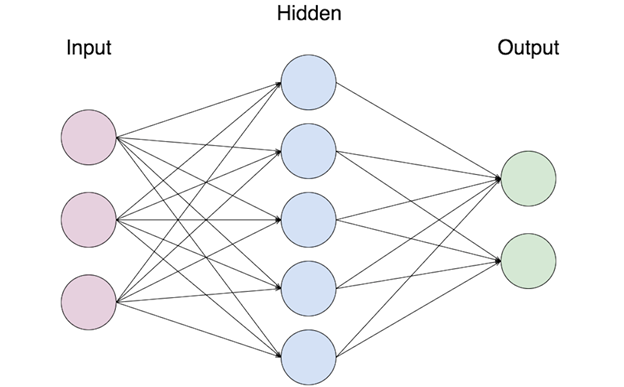
\includegraphics[width=\columnwidth]{fig8.png} 
	\caption{Visual representation of a Neural Network.}
\end{figure}

\begin{figure}[h]
	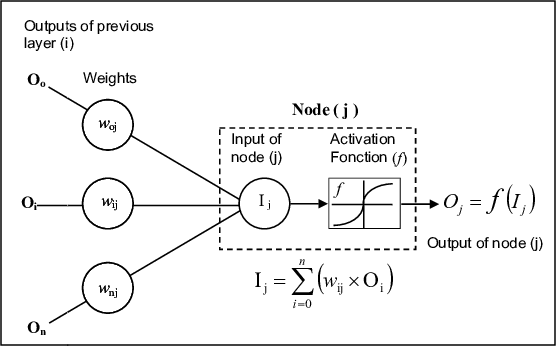
\includegraphics[width=\columnwidth]{fig9.png} 
	\caption{(Chokmani, Khalil, Ouarda, \& Bourdages, 2007) forward propagation through a single neuron is depicted.}
\end{figure}
\paragraph{Forward propagation}
In Figure 9, the inputs on the left-hand side are the outputs of all neurons of the earlier layer or constitute the vectorised input from the environment to the network (input layer). Based on the output of the last layer conclusions on the input are drawn (Schmidhuber, 2016) and is called the output layer. Every layer between the output and the input layer are called hidden layers. Each node multiplies all its inputs with a weight respectively, takes the sum of this (Ij), and this creates the input for the activation function (f). The output of the activation function (Oj) is a single number, serves as the output of the single node, and creates part of the input for the next layer of neurons. The activation function ensures that the output of the neuron lies in the desired range and creates a non-linear system. Only then is the network able to solve non-trivial problems with complex solutions, otherwise, it would only compute a linear function Wx of the input x, no matter how deep the network is (Goodfellow et al., 2016). For binary classification problems, the sigmoid function is widely used, as seen in Figure 9. (TechnoReview, 2013)

\paragraph{Back-Propagation}
The weights that are multiplied with input of the node are adjusted in the backpropagation through the network. In backpropagation the weights in the network are commonly adjusted according to the first order derivative of the cost function (expected return) with respect to the parameters of the model, like square meters, number of rooms, and number of bathrooms are parameters when determining the price of a house. The aim of any algorithm is to maximise the cost function, its goal is determined by how this cost function is defined. Algorithms that directly adjust their weights according to the cost function are called policy-based learning algorithms (Goodfellow et al., 2016).

\subsubsection*{Convolutional Neural Networks (CNN)}
\textit{Information extracted from Convolutional Neural Networks on Coursera by Ng (2018) and Deep Learning by Goodfellow et al. (2016).}

CNNs are able to process images and frames of videos with a slightly different set-up than regular neural networks. The CNN takes in a matrix representation of the picture or frame of the video. The matrix representation stores the intensity of a certain colour in every pixel for every pixel. With greyscale input, there is only one matrix and a full-colour input has a representation of three matrices stacked on top of each other, red, green, and blue respectively. These matrices are processed in two ways in one convolution layer, namely using convolution and pooling. 

\begin{figure*}[h]
	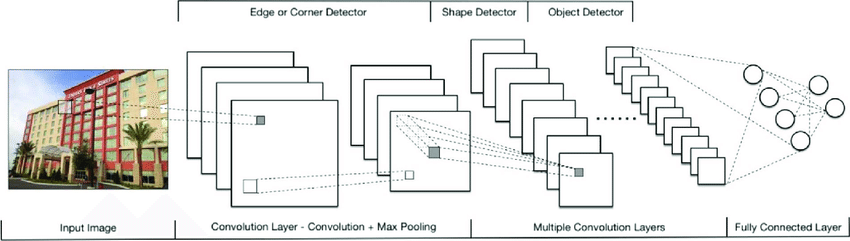
\includegraphics[width=\textwidth]{fig10.png} 
	\caption{Layers of a CNN (Ma, Xiang, Du, \& Fan, 2018).}
\end{figure*}

\paragraph{Forward Propagation}
Convolution
The convolution uses a smaller matrix, a so-called `mask`. This mask is depicted as the small square in Figure 10 of the building and it builds up the values in the second matrix as the mask moves from the top left, over the whole picture, to the bottom right. The mask always uses the same depth dimension as the input and there are often multiple different masks applied in one convolution step. The mask contains certain variable weights. When the mask is laid over a specific part of the image it multiplies the values of that point in the matrix, adds all the outcomes up and this becomes the value in the next matrix. 

\paragraph{Pooling}
Pooling is done per section of the matrix and has multiple versions. This section does not slide across the matrix but separates the matrix into specific parts. Widely applied versions of pooling are average pooling and max pooling. Pooling has a similar function as to the activation function in a neural network, applying non-linearity to the system, allowing it to produce complicated networks and relations. Pooling happens from the second to the third matrix in Figure 10. It takes a defined section of the matrix and builds the third matrix by either taking the average (average pooling) or maximum (max pooling) of the values in this section. 
\begin{figure*}[h]
	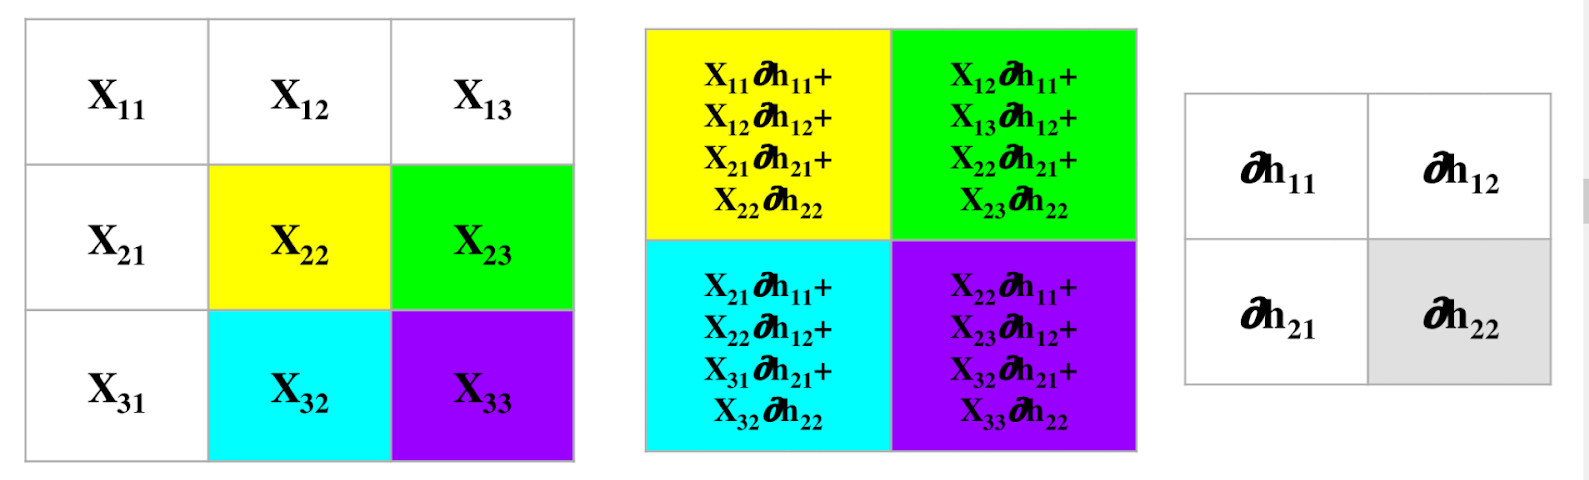
\includegraphics[width=\textwidth]{fig11.png} 
	\caption{(Agarwal, 2017), the derivative of the cost function just as a normal neural network but it updates the value according to the sum of the derivatives of the cost function (shown in the middle matrix) with respect to each value that is taken into account by a specific value in the mask (first matrix)}
\end{figure*}
\begin{figure}
	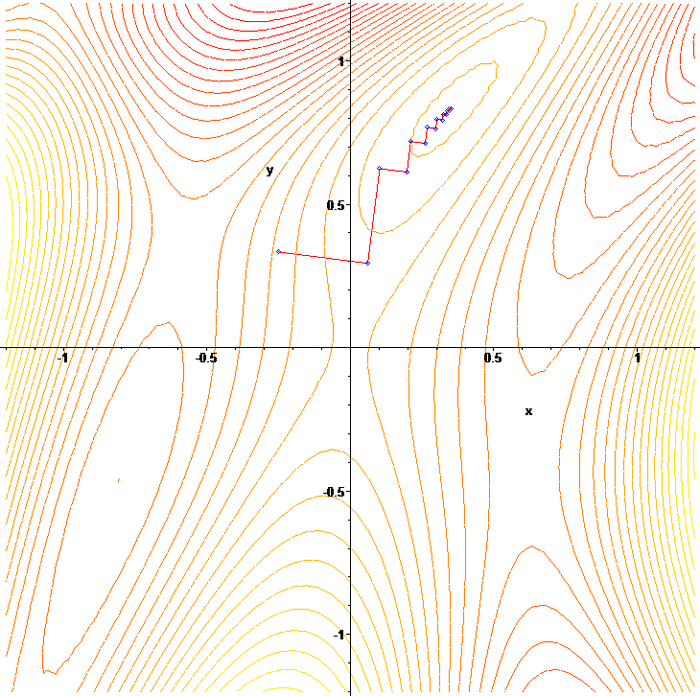
\includegraphics[width=\columnwidth]{fig12.png} 
	\caption{(Gillis, 2006), creating an algorithm that maximises more precisely and  efficiently using $2^{nd}$ order optimisation .}
\end{figure}
\paragraph{Convolution layer and progress through the network}
After proceeding through the first layer, explained by the steps above, the next convolution layer then scans over the results of the pooling of the earlier layer, executes the convolution, and pools them. The matrices shrink in the convolution step under the influence of the size of the mask and the `stride`. The stride is the step size with which the mask moves across the earlier matrix. In the pooling layer, the matrix shrinks under the influence of the size of the sections. 
After running the desired number of convolutional layers with the desired settings, the matrix is flattened out into one long vector. This vector is then processed by fully connected layers which are essentially the same as the neural network described before but take the output of the convolutional layers as input. This then serves to identify objects in the image, select a preferred action given the image, or recognise faces, depending on the goal of the network.

\paragraph{Back-Propagation}
In the backward propagation of the CNN, the values of the masks (middle and last matrix) are updated. The values of the mask are comparable to the weights of a simple neural network. The values of the mask are then updated according to the

\subsubsection*{Optimization} 
Optimization practically determines in which direction the algorithm is going to shift its values with the goal to minimise the loss function, eventually guiding the network to an optimal policy.
$1^{st}$ order optimization updates the value using the first order derivative of the `cost` function. The weight is updated by adding the first order derivative multiplied by the set learning rate to the weight. The first order derivative provides the slope at every point of the plane of the cost function

$2^{nd}$ order optimization is a very computationally expensive process when this is done with the exact values. The $2^{nd}$ order statistic of the cost function, however, enables the algorithm to make an accurate estimation of how the cost can be maximised in the most efficient and certain way. The second order statistic determines how confident it is that a step in a certain direction will get it to maximise the cost function. This can then be used to determine the direction of the step and the magnitude of the step with more precision, smoothening the trajectory depicted in Figure 12  Therefore multiple different methods attempt to approximate this $2^{nd}$ order statistic of the cost function. 

\subsubsection*{Difference between policy-based and value-based learning}
Apart from the policy-based learning algorithms, there are value based learning algorithms. These algorithms are trained to estimate the value of a variable given a certain state from the environment it is evaluating. This algorithm cannot directly update its parameters since it is concerned with estimating a value that lies in the future (time + 1). It cannot calculate a cost function because it needs the next run to determine whether its estimation was accurate and only then can the algorithm update its weights (Sutton \& Barto, 1998; McClelland, 2015). The remaining process of learning of value-based learning algorithms is similar to what was described earlier.


\begin{table*}[h]
	\begin{tabular}{ |l|p{5cm}p{5cm}|  }
		\hline
		Device                  & \thead{1}                                      & \thead{2}                                     \\ \hline
		Device name             & Lenovo Thinkpad P51                                        & Dell Inspiron 15 gaming 7567                              \\
		Processor               & Intel(R) Core$^{TM}$ i7-7700HQ cpu @ 2.80GHz, 2808 Mhz         & Intel(R) Core$^{TM}$ i7-7700HQ cpu @ 2.80GHz, 2808 Mhz        \\
		Random Access Memory    & 16GB / 2400MHz DDR4, non-ECC                               & 16GB / 2400MHz DDR4, non-ECC                              \\
		Primary Graphics Card   & NVIDIA Quadro M1200 (4096MB; CUDA compute capability: 5.0) & Nvidia GTX 1050-Ti (4096 MB; CUDA compute capability 6.1) \\
		Secondary Graphics Card & Intel(R) HD Graphics 630                                   & Intel(R) HD Graphics 630                                  \\ \hline
	\end{tabular}
\caption{Device Hardware Specifications}
\end{table*}

\begin{table*}[]
	\begin{tabular}{ll}
		\hline
		\multicolumn{2}{c}{Software set-up} \\
		\hline
		Operating System: & Linux Ubuntu 18.10 (same on both devices) \\
		Graphics driver: & Nvidia driver 396.54 (same on both devices) \\
		CUDA: & CUDA 9.0 (Same on both devices) \\
		Python: & 3.6.3 (device 1), 3.6.6 (device 2) \\
		Dependencies: & See requirements.txt (Gopal, van der Neut, 2018) \\
		\hline
	\end{tabular}
\caption{Software Setup for the study}
\end{table*}

\begin{table*}[]
	\begin{tabular}{|p{7cm}|p{7cm}|}
		\hline
		\thead{Device 1} & \thead{Device 2} \\ \hline
		- & PPO2 on SpaceInvaders x2 and Pong x1 \\ \hline
		ACKTR on SpaceInvaders x2 & PPO2 on Pong and DemonAttack x2 \\ \hline
		ACKTR on DemonAttack x2 & PPO2 and ACKTR base SpaceInvaders on Pong \\ \hline
		ACKTR on Pong x2 & ACKTR base SpaceInvaders on DemonAttack x2 \\ \hline
		ACKTR on Q*Bert x2 & PPO2 base SpaceInvaders on Q*Bert x2 \\ \hline
		ACKTR base SpaceInvaders on Q*Bert x2 & PPO2 base SpaceInvaders on DemonAttack x2 \\ \hline
		ACKTR base Q*Bert on SpaceInvaders x2 & PPO2 base Q*Bert on SpaceInvaders x2 \\ \hline
		ACKTR base Q*Bert on Pong x2 & PPO2 base Q*Bert on Pong x2 \\ \hline
		ACKTR base Q*Bert on DemonAttack x2 & PPO2 base Q*Bert on DemonAttack x2 \\ \hline
		ACKTR base Pong on SpaceInvaders x2 & PPO2 base Pong on SpaceInvaders x2 \\ \hline
		ACKTR base Pong on Q*Bert x2 & PPO2 base Pong on Q*Bert x2 \\ \hline
		ACKTR base Pong on DemonAttack x2 & PPO2 base Pong on DemonAttack x2 \\ \hline
		ACKTR base DemonAttack on SpaceInvaders x2 & PPO2 base DemonAttack on SpaceInvaders x2 \\ \hline
		ACKTR base DemonAttack on Q*Bert x2 & PPO2 base DemonAttack on Q*Bert x2 \\ \hline
		ACKTR base DemonAttack on Pong x2 & PPO2 base DemonAttack on Pong x2 \\ \hline
		ACKTR base SpaceInvaders on SpaceInvaders, ACKTR base DemonAttack on DemonAttack & PPO2 base SpaceInvaders on SpaceInvaders, PPO2 base DemonAttack on DemonAttack \\ \hline
		ACKTR base Pong on Pong, ACKTR base Q*Bert on Q*Bert & PPO2 base Pong on Pong, PPO2 base Q*Bert on Q*Bert \\ \hline
	\end{tabular}
\caption{Training runs per device in chronological order}
\end{table*}


\subsection*{B}
\begin{itemize}
	\item Hardware Specifications: Table 5
	\item Software Setup: Table 6
	\item Training Runs per device in chronological order: Table 7
	\item Hyperparameters: Table 8
	\item Graphs of Raw Data: Figure 13
\end{itemize}

\begin{table*}[]
	\begin{tabular}{l|ll}
		\hline
		\thead{Hyperparameters} & \thead{PPO2} & \thead{ACKTR} \\
		\hline
		Network & Nature CNN & Nature CNN \\
		nsteps & 2048 & 20 \\
		Discount & 0.99 & 0.99 \\
		GAE parameter (λ) & 0.95 & 0.95 \\
		Learning rate & 3.00E-04 & 0.25 \\
		VF coeff.c1(9) & 0.5 & 0.5 \\
		Entropy coeff. c2(9) & 0 & 0.001 \\
		Clipping parameter & 0.2 & (KFAC) 0.001 \\
		Noptepochs & 4 & - \\
		Numprocs & - & 32 \\
		VF fisher coeff & - & 1 \\
		Number of actors & - & 8 \\
		Lr schedule & - & linear \\
		\hline
	\end{tabular}
\caption{Hyperparameters as extracted from OpenAI Baselines(2018).The terms do not necessarily carry same meaning for both algorithms.}
\end{table*}

\begin{figure*}[b]
	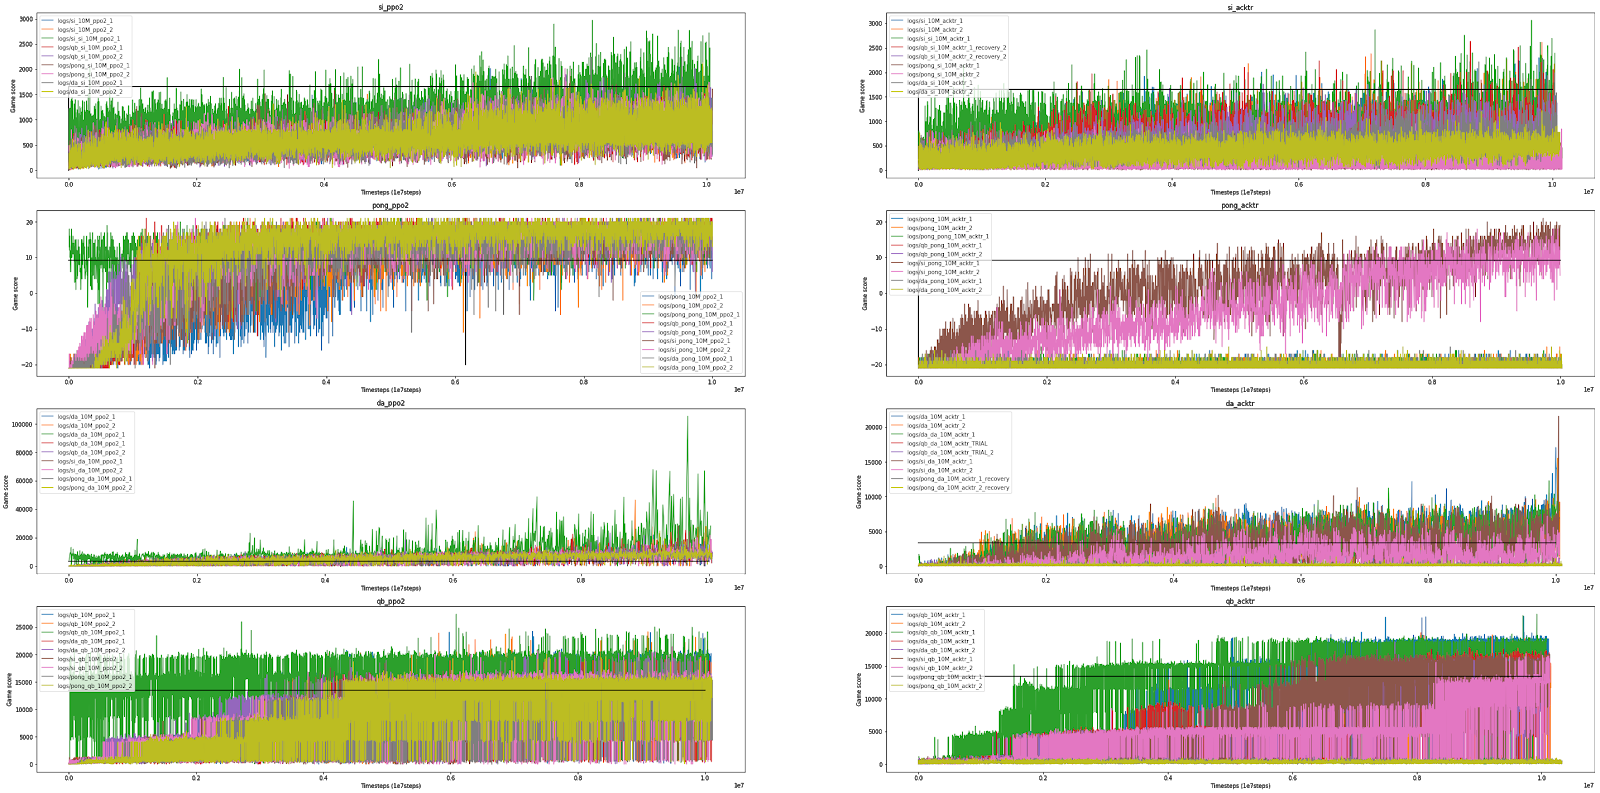
\includegraphics[width=\textwidth]{fig13.png} 
	\caption{Game score(Raw data) at each timestep during the 10M timesteps }
\end{figure*}
\end{document}
